% $Id$

\chapter{Multi-modal face recognition example}
\label{sec:multimodal_face}
\minitoc

The dataset used in this tutorial consists of is a visual experiment where pictures of famous faces (Famous), unfamiliar faces (Unfamiliar) and scrambled faces (Scrambled) are presented to the subjects. In total 16 subject were recorded with fMRI, EEG and MEG. The data is available for research purposes from ftp://ftp.mrc-cbu.cam.ac.uk/personal/rik.henson/wakemandg\_hensonrn/ and is fully detailed in the publication: \textit{‘A multi-subject, multi-modal human neuroimaging dataset’, Wakeman, D. G. and R. N. Henson, Scientific Data, vol. 2, 150001, 2015.}
\\

A within-subject version of the dataset can be found, along with pre-processing batches, on the SPM website (https://www.fil.ion.ucl.ac.uk/spm/data/mmfaces/).
\\

In this tutorial, the EEG and MEG data was used to derive 6 modalities:

\begin{itemize}

\item MEG: average trace for each channel, in the considered time window. There are 102 MEG channels. There is one file with the 3 traces per subject.
\item Interpolated EEG: nifti images from spatial interpolation of average trace per condition on the scalp, for EEG. We thus obtain one image per condition and per subject.
\item Interpolated MEG: nifti images from spatial interpolation of average trace per condition on the scalp, for MEG.
\item Connectivity EEG: for each pair of channels, we computed the correlation between the average traces of a condition. The output is a 70*70 matrix per condition and per subject. Only the upper triangular part of the matrix was extracted.
\item Connectivity MEG: for each pair of channels, we computed the correlation between the average traces of a condition. The output is a 102*102 matrix per condition and per subject. Only the upper triangular part of the matrix was extracted.
\end{itemize}

The EEG, MEG, interpolated EEG and MEG files were obtained from following the batches provided with the corresponding chapter in the SPM manual. The connectivity was built from the obtained EEG and MEG files, based on in-house scripts (in the Appendix).

% \begin{figure}[!h]
% 	\centering
% 	\begin{minipage}[b][7cm][b]{0.5\textwidth}
%   \centering
% 		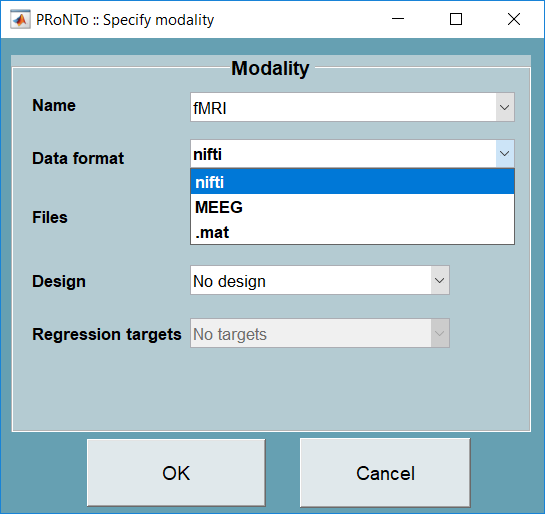
\includegraphics[scale=0.5]{images/Tutorial/v3/data_example1/gui_data_and_design_modality_data_format.png}
% 		  \captionsetup{width=0.9\linewidth}
% 	\captionof{figure}{`Specify modality' GUI. First we specify the format of our data (here nifti).}
% 	\label{fig:gui_data_and_design_modality_data_format}
% \end{minipage}%
% 	\begin{minipage}[b][7cm][b]{0.5\textwidth}
%   \centering
% 		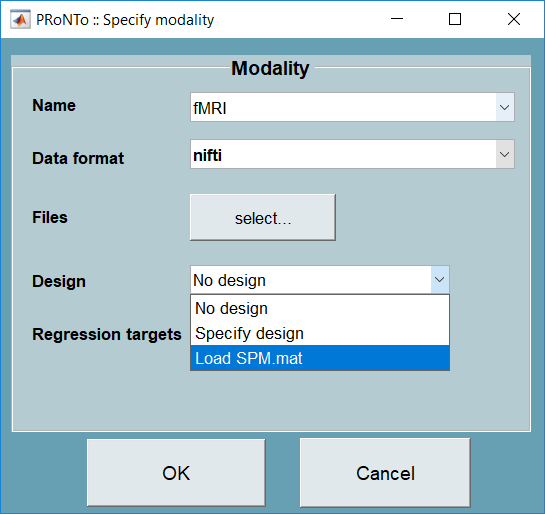
\includegraphics[scale=0.5]{images/Tutorial/v3/data_example1/gui_data_and_design_modality_specify_design.png}
% 		\captionsetup{width=0.9\linewidth}
% 	\captionof{figure}{`Specify modality' GUI. Here we load a specified design from an `SPM.mat' file.}
% 	\label{fig:gui_data_and_design_modality_specify_design}
% 	\end{minipage}
% \end{figure}


\section{GUI analysis}

We will first analyse the data using PRoNTo's GUI and then repeat the analysis using the {\tt matlabbatch} system. As this is a much more complex tutorial, readers are strongly advised to go through the other tutorials first to get a better understanding of PRoNTo's functionalities. Also, since this is the fourth tutorial, some parts that have been previously described will be only shortly described here. Therefore, the reader is advised to go through the previous tutorials first.
\\

To start, create a new directory in which to save the results of the analysis, then start up \matlab{} and type `prt' or `pronto' in the \matlab{} prompt. This will open the main interface of PRoNTo.

\subsection{Data \& design}

There are 16 subject to input. For each subject, there are 6 modalities to specify. The easiest way to do this is to fully specify subject 1, then use the entered modalities and designs in further subjects.


\begin{itemize}

\item Choose a directory to save the resulting PRT.mat.
\item Add a group (e.g. `G1'), one subject (`S1'), and leave the `Samples' tick box below the panel unchecked. See Chapter \ref{chap:DataDesign} of the manual for more information on this option.

\end{itemize}

\noindent \textbf{\underline{EEG/MEG (MEEG data format)}}

\begin{itemize}

\item The first modality to be specified will be the EEG. Provide the name `EEG' and choose its type as `MEEG'. The MEEG data formats usually consist of two files, one $.mat$ and one $.dat$. In this case we have to go to $/Multimodal\_face\_dataset/data/S1/EEG$ where we'll find the EEG data of the first subject (`S1').

\item When the file is selected, PRoNTo will automatically read the design from it. The design can be reviewed be clicking on `Events in file'.

In Figure \ref{fig:multimodal_face_gui_data_and_design_specify_modality_and_conditions} we see both the MEEG modality specification in mention, and the MEEG design review. There we see 3 conditions: Unfamiliar, Famous and Scrambled. The units are already set to seconds and the TR is the sampling interval (in seconds) in the file. In this example, the TR of 0.005 corresponds to a sampling rate of 200Hz.

\begin{figure}[!h]
  \centering
		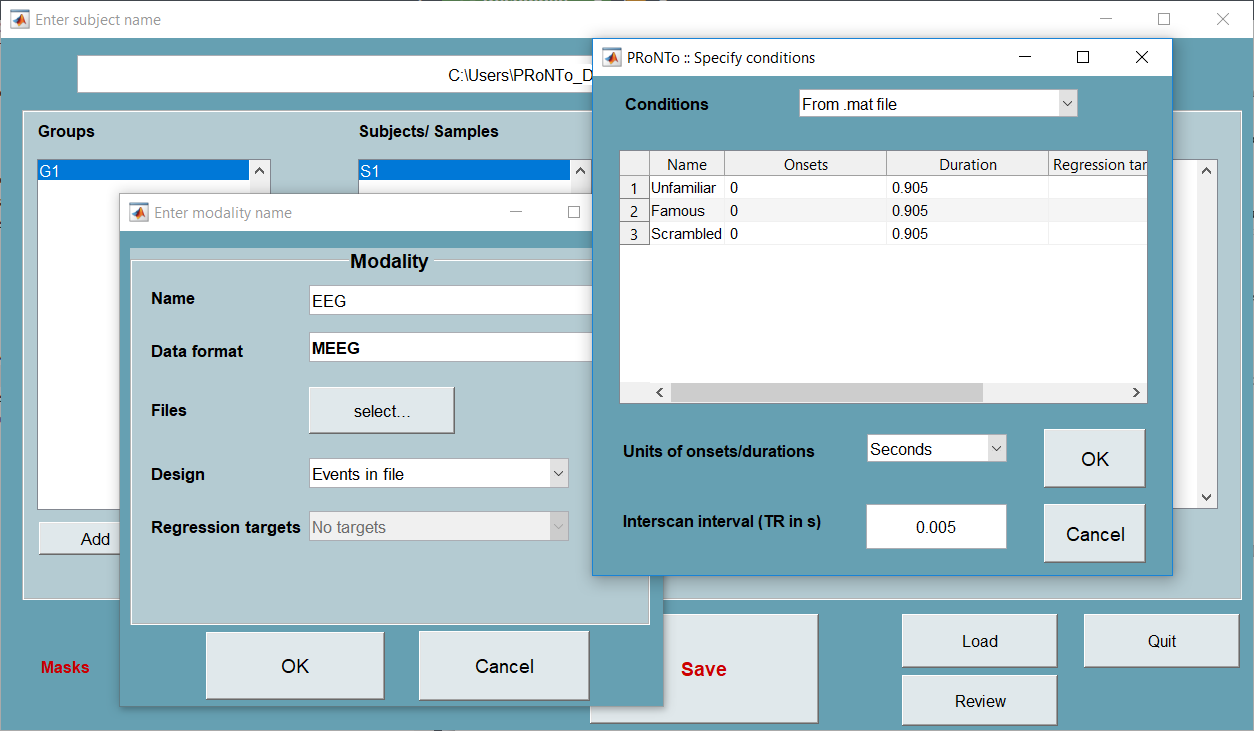
\includegraphics[scale=0.6]{images/Tutorial/v3/multimodal_face_tutorial/multimodal_face_gui_data_and_design_specify_modality_and_conditions.png}
	\caption{`Specify modality' and `Specify conditions' GUIs.}
	\label{fig:multimodal_face_gui_data_and_design_specify_modality_and_conditions}
\end{figure}

\item The same can be done for the MEG modality, where you will only have to change the name and choose the appropriate MEG files, instead of the EEG files that we chose before.

\end{itemize}

\noindent \textbf{\underline{Interpolated EEG/MEG (nifti data format)}}

\begin{itemize}

\item The interpolated EEG and MEG consist of nifti files. This is similar to entering beta images from a GLM analysis in previous versions of PRoNTo. The only difference is that the type now needs to be specified; even though nifti is the default option.

\item In the `Specify modality' GUI, provide a name to the modality, e.g. `interpEEG', choose `nifti' and select the appropriate files, which are found in $/Multimodal\_face\_dataset/data/S1/EEG\_interp$. As there are 3 conditions, we have 3 different files, one for each condition.

\begin{itemize}
\item \noindent \textbf{Very important note}: the order you choose the conditions (their files) should be the same across all modalities that will be used in a single model. This means that we should use the same order (Unfamiliar, Famous, Scrambled) that was input with the EEG and MEG files.
\end{itemize}

\item Since there is no SPM.mat file for the design, we need to specify the design ourselves.

\begin{itemize}
\item Create a new design by selecting the option `Specify design'.
\item If we do not have a .mat file with the design information, we need to specify the experimental design manually. Select the `Specify' option in the `Specify conditions' GUI. First you need to write how many conditions you have, which in this case is 3 (corresponding to the 3 image files).  This will open another window that allows the user to write the names, onsets and durations of each condition.

\item As when using beta images, the onsets should correspond to the index of the image in the file selection, with the smallest index (i.e. first selected image) being 0. The duration should be set to 1 for all images, and the units should be set to `Scans', with a TR of 1. Take great care when specifying conditions manually. The initial and final `Specify conditions' window should look similar to the one in Figure \ref{fig:multimodal_face_gui_data_and_design_specify_conditions_nifti}.

\begin{figure}[!h]
  \centering
		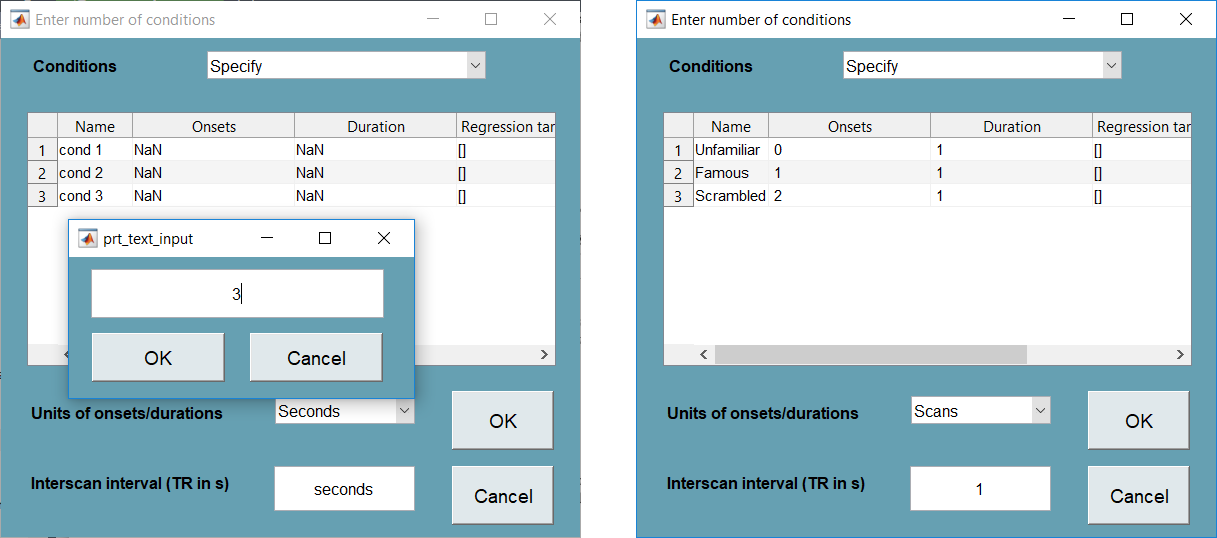
\includegraphics[scale=0.6]{images/Tutorial/v3/multimodal_face_tutorial/multimodal_face_gui_data_and_design_specify_conditions_nifti.png}
	\caption{`Specify conditions' GUI and final configuration.}
	\label{fig:multimodal_face_gui_data_and_design_specify_conditions_nifti}
\end{figure}

\end{itemize}

\item The same can be done for the interpolated MEG modality, where you will only have to change the name (`interpMEG') and choose the appropriate MEG files, instead of the EEG files that we chose before.
\end{itemize}

\noindent \textbf{Note:} If we have many subjects and many conditions, this procedure can be tiresome and is quite prone to mistakes. Therefore what one could do is manually create a `Design.mat' file and include the information regarding the names, onsets and durations inside that file. The name of the .mat file itself is irrelevant. What is important is to have 3 different cell arrays named `names', `onsets' and `durations'. The dimensions of all 3 cell arrays should be 1 x \#conditions. So in our case all 3 cell arrays will have 1x3 dimensions for the 3 conditions (Unfamiliar, Famous, Scrambled). You can find one such example design file called `Design.mat' in the $/Multimodal\_face\_dataset/data$.
\\

So for the interpolated MEG modality and from now on, do not input manually all the conditions in the `Specify conditions' GUI. Instead, select the `From .mat file' option and choose the `Design.mat' file located in the $/Multimodal\_face\_dataset/data$ folder. As you can see one still needs to choose the `Units of onsets/durations' and the `Interscan Interval' options. So again set the units to `Scans', and the TR to 1.
\\

\noindent \textbf{\underline{Connectivity EEG/MEG matrices (.mat data format)}}

\begin{itemize}

\item Finally we have the connectivity derived EEG and MEG matrices, which can be entered in a similar way as for images. We set the name as `ConnEEG'.
\item The `Data format' needs to be set to `.mat'. The files in this case are `.mat' files, and usually we will have 1 file for each condition, hence 3 for each subject. The order with which we input the files needs to be the same as before (Unfamiliar, Famous, Scrambled).

\item The possible design options are then ‘Specify design’ or ‘No design’. Specifying the design is identical to that of (nifti) images. As for images, PRoNTo expects one .mat file per trial/sample. \textbf{Important note:} When loading the file, it will read the first variable only (independently of the variable’s name). You hence need to ensure that the variable of interest is saved as the first one, or in a specific .mat. For ease of use, keep using the last way we mentioned to specify conditions (using the design file called `Design.mat' in the $/Multimodal\_face\_dataset/data$).

\item The same can be done for the connectivity MEG modality, where you will only have to change the name (`ConnMEG') and choose the appropriate MEG files, instead of the EEG files that we chose before.


At this point we have finished inputting the first subject\footnote{For the more experienced users we have included a small \matlab{} script inside the $/PRoNTo\_main\_folder/manual$ called `16\_script.m' that automatically creates the rest of the subjects provided you have followed exactly the same steps as the ones mentioned in the tutorial, you have completely finished the first subject, you have specified the interpolated EEG and MEG masks and you have saved the struct. You need to load the `PRT.mat', and be sure you're in the same directory of your `PRT.mat'.}. 

\begin{itemize}
\item You can now start the second subject. You first create a new subject, e.g. `S2'.

\item The modalities of the second subject can then be entered by selecting the already specified modalities, where first you will need to select the appropriate data files of that subject, those of the second subject instead of the first one we selected before.

\item You will also need to specify the design wherever you specified it manually. So for EEG and MEG, the design is read automatically. For nifti and .mat data formats, a new option will appear in the `Design' menu of the `Specify modality' GUI. The `Design' menu will have the extra option `Replicate design from subject 1', that is very convenient in this application. You can of course re-specify it manually again by locating the design file called `Design.mat' in the $/Multimodal\_face\_dataset/data$, as we did before. You will need to do this for all 16 subjects.
\end{itemize}

\item Finally we need to specify the masks. While mask files definitely need to be specified for nifti images, for .mat and MEEG data formats, we indeed assume that the data only contains relevant features (therefore there is no need for a mask), as this can be easily performed during pre-processing. Please ensure that your data (.mat or MEEG) do not contain NaNs.

If the user wants to use a mask, it can still be done at the feature set level (for connectivity matrices, we'll see in another tutorial that another option could be to enter the full matrix and specify a 2nd level mask).

\end{itemize}

After you have specified everything, the final configuration should look like the one in figure \ref{fig:multimodal_face_gui_data_and_design_final}, with 16 subjects, each one with its 6 modalities.

\begin{figure}[!h]
  \centering
		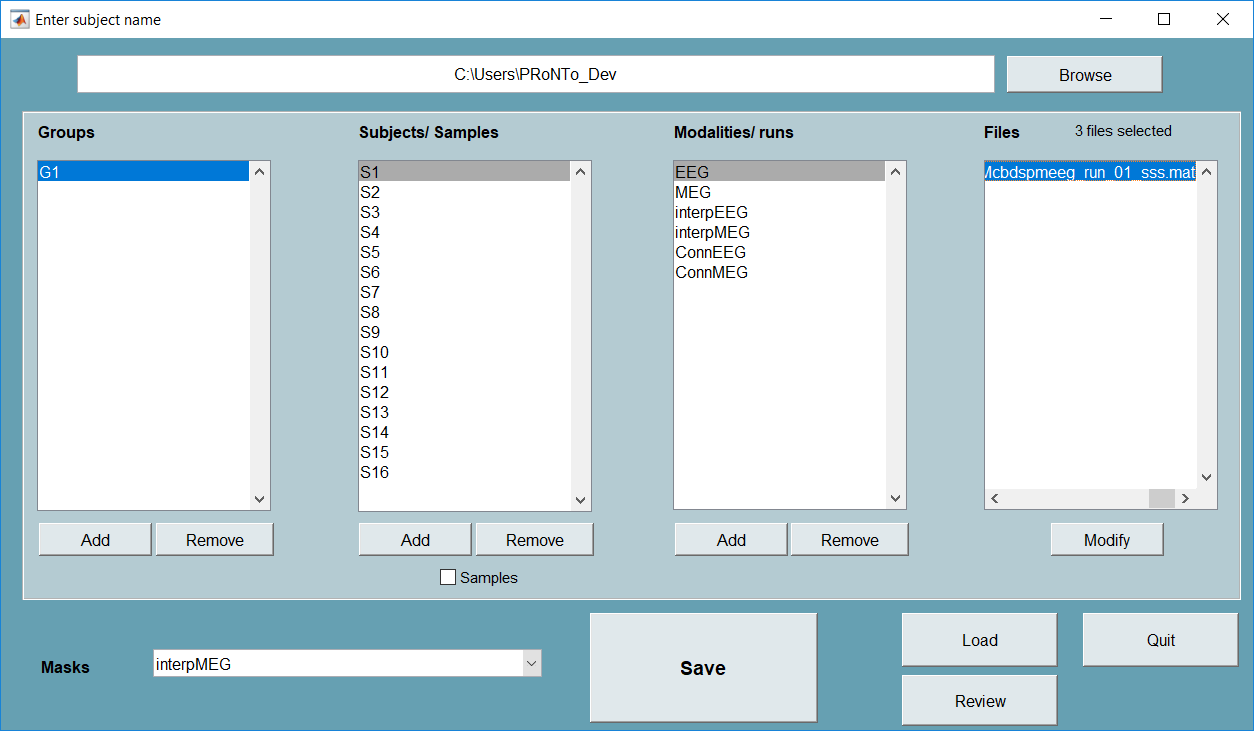
\includegraphics[scale=0.6]{images/Tutorial/v3/multimodal_face_tutorial/multimodal_face_gui_data_and_design_final.png}
	\caption{`Data \& Design' GUI final configuration.}
	\label{fig:multimodal_face_gui_data_and_design_final}
\end{figure}

\textbf{Note regarding NaN values:} A simple `Check Reg' in SPM will show that the interpolated EEG (MEG) images have NaNs at different pixels, for different subjects. We hence need to create a common mask to discard those NaNs. This can easily be performed using SPM \textit{ImCalc} batch (select all images from the EEG interpolated modality, select `read as matrix', operation can be: \textit{~isnan(sum(X))} ) and should be done for EEG and MEG separately.
\\

\noindent \textbf{Understanding the `PRT' structure:} At this point we have a `PRT.mat' in the directory you previously chose. It would be quite useful to load this in \matlab{} and take a look at its structure, in order to start familiarizing yourself with how PRoNTo structures everything. Once you slowly start being comfortable with this, you will start to understand its great practicality. Maybe for example you want to inspect something you did and you are not sure of, and maybe there is no explicit way to inspect this through the available GUIs. Instead of re-doing everything right from the start, you can inspect `PRT.mat' directly from the \matlab{} Workspace.
\\

For example, if you load the `PRT.mat' file that was created and you go inside the `PRT.group' field, you will see a field called `gr\_name' which only has one group, `G1', and another field called `subject' whose value is 1 x \#subjects. If you now go inside `subject', you will notice two different fields. Now we are inside the subjects of `G1'. Here you can see one field with the name `subj\_name' where we can see the 16 different subjects we created, and another field called `modality' which includes the 6 different modalities for each subject. Go further inside if you wish, to the `modality' field of `S1'. Here you see 6 entries (one for each modality), each of which has 6 fields, `mod\_name' which includes the names we input, `covar' which includes possible covariates, `rt\_subj' which includes potential regression targets, `design' which includes the designs we input, `scans' which includes the data files we input for each subject and finally `type' which is the data format of each data file. That way you can easily check in a direct manner what you have input in every step you did previously.
\\

Learning to explore and manoeuvre around the `PRT.mat', while not obligatory, will definitely help you a lot and make your life much more practical. It can save you from potential typo or other types of mistakes because it's an easy and fast way to check your inputs. So we strongly advise readers who intend to make heavy use of PRoNTo to start familiarizing themselves with the \matlab{} Workspace and the main PRoNTo structures and even write their own \matlab{} scripts automating some of the trivial procedures, like the one we did. A \matlab{} script is a much safer way to process mundane tasks that require a lot of mouse clicks which can be tiresome and quite prone to human errors.
\\

As in the previous tutorials the design can be reviewed. If properly specified, it will display one group of 16 subjects, with 6 modalities. For nifti modalities, this is where you would specify HRF parameters if you were using a design specified in seconds. This option is (obviously) not available for .mat or MEEG. In the present case, our design is in terms of images/scans. The default values of 0 and it should not be modified. The `Review data' GUI would look like Figure \ref{fig:multimodal_face_gui_data_and_design_review}.

\begin{figure}[!h]
  \centering
		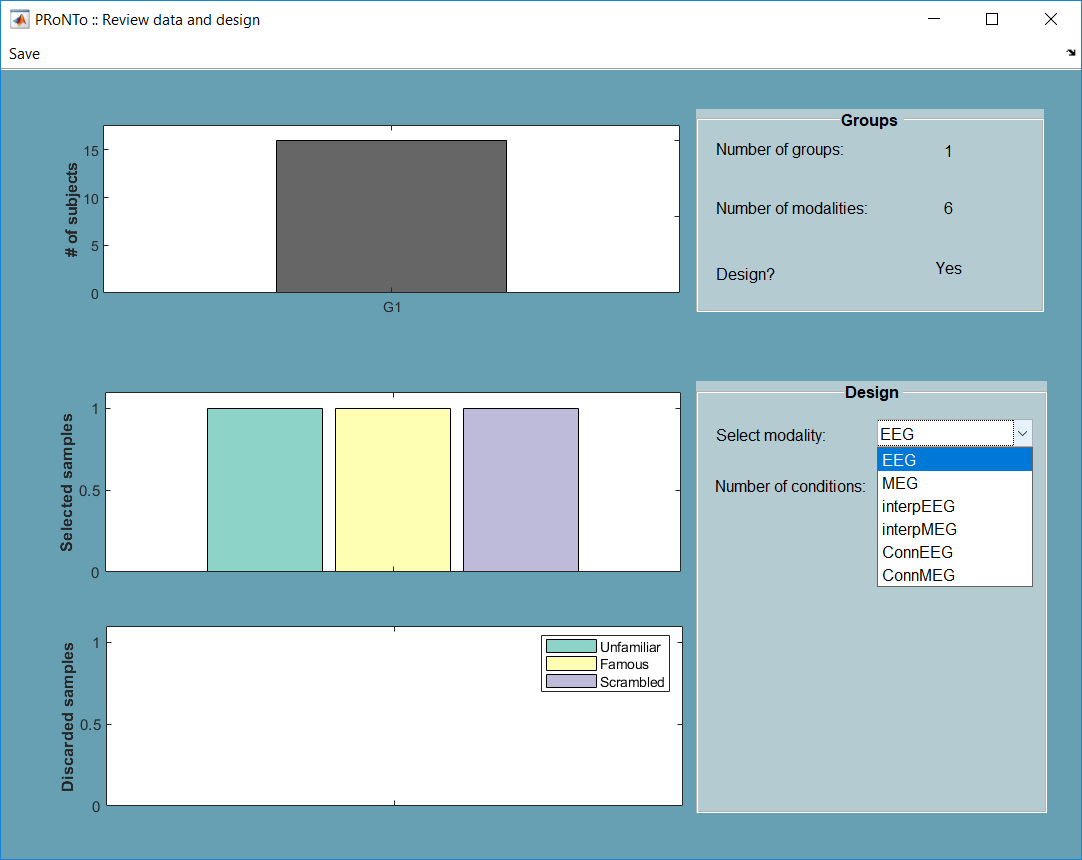
\includegraphics[scale=0.6]{images/Tutorial/v3/multimodal_face_tutorial/multimodal_face_gui_data_and_design_review.png}
	\caption{`Review data' GUI.}
	\label{fig:multimodal_face_gui_data_and_design_review}
\end{figure}

%------------------------------------------------------------------

\subsection{Prepare feature set}

In versions 2.X, modalities could be combined in 2 ways at this stage: either concatenated in samples (e.g. multiple runs of a same experiment), or by computing one kernel per modality and storing them together. This had the limitation that combined modalities (in either way) had to have the exact same number of features. We have now decoupled those operations for more flexibility. At the feature set stage, modalities can only be concatenated in samples. In this case they still need to have the exact same number of features.
\\

As we want to use our modalities as different `features’ for the same model and not as different samples, we hence need to build one feature set per modality. The different data types are handled in different ways: images and .mat in a way similar to v2, MEEG with a new window. This means that, after loading the `PRT.mat' in the `Prepare feature set' GUI, a new window like the one in figure \ref{fig:multimodal_face_gui_prepare_featureSet_specify_data_type} will appear if multiple data formats are contained in the `PRT.mat'. The window asks which data format the specified feature set will have. Feature sets are built for only one data format at a time. The buttons available on this interface will reflect the data formats present in your PRT. If only one type is present, this step is skipped.

\begin{figure}[!h]
  \centering
		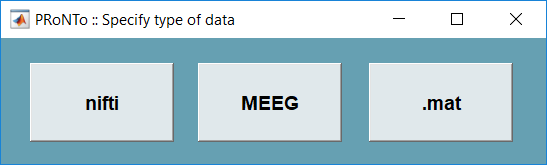
\includegraphics[scale=0.65]{images/Tutorial/v3/multimodal_face_tutorial/multimodal_face_gui_prepare_featureSet_specify_data_type.png}
	\caption{`Specify type of data' GUI}
	\label{fig:multimodal_face_gui_prepare_featureSet_specify_data_type}
\end{figure}

\noindent \textbf{\underline{Interpolated EEG/MEG (nifti data format)}}

\begin{itemize}

\item We first choose `nifti' and will build the feature set for interpolated EEG. Once the data format has been chosen, the process is similar to that of v2: if there are multiple modalities of that data format in the PRT, the left window of figure \ref{fig:multimodal_face_gui_prepare_featureSet_prepare_featureSet} will appear, asking how many modalities to concatenate. Here, there is only one modality to consider.

\item After specifying `1' and `Enter/Return', the appropriate window, like the one in figure \ref{fig:multimodal_face_gui_prepare_featureSet_specify_modality} will then open to specify parameters for this specific modality. If there were multiple modalities to concatenate, the following windows would open as many times as the number entered.

\begin{figure}[!h]
	\centering
	\begin{minipage}[b][8.8cm][b]{0.5\textwidth}
  \centering
		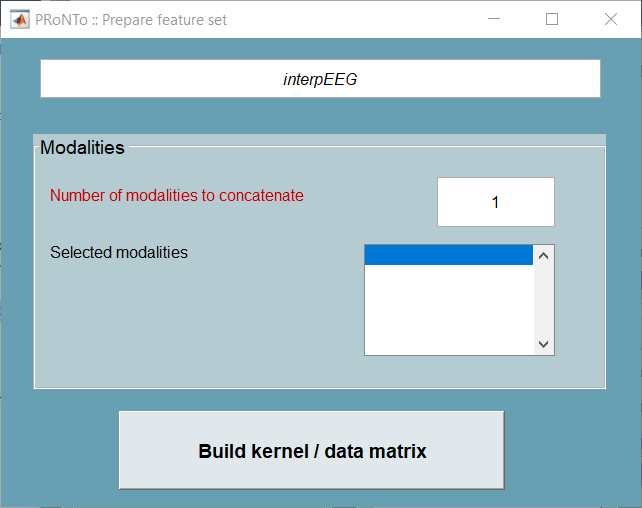
\includegraphics[scale=0.6]{images/Tutorial/v3/multimodal_face_tutorial/multimodal_face_gui_prepare_featureSet_prepare_featureSet.png}
		  \captionsetup{width=0.9\linewidth}
	\captionof{figure}{`Prepare feature set' GUI.}
	\label{fig:multimodal_face_gui_prepare_featureSet_prepare_featureSet}
\end{minipage}%
	\begin{minipage}[b][8.8cm][b]{0.5\textwidth}
  \centering
		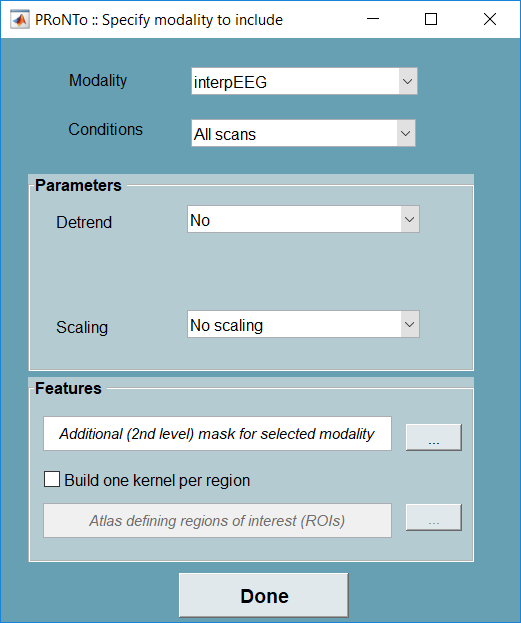
\includegraphics[scale=0.6]{images/Tutorial/v3/multimodal_face_tutorial/multimodal_face_gui_prepare_featureSet_specify_modality.png}
		\captionsetup{width=0.9\linewidth}
	\captionof{figure}{`Specify modality' GUI.}
	\label{fig:multimodal_face_gui_prepare_featureSet_specify_modality}
	\end{minipage}
\end{figure}

\item For nifti images, the whole process as we know it from versions 2.X and from the previous tutorials is the same. All options previously available are included in v3, with no addition. We select all default options. We then repeat the same procedure for the interpolated MEG modality (`interpMEG') to create a second feature set.

\end{itemize}

\noindent \textbf{\underline{Connectivity EEG/MEG (.mat data format)}}

\begin{itemize}
\item To create the connectivity EEG/MEG feature sets, we repeat the first step but select `.mat'. As we have 2 .mat modalities (EEG and MEG), window in Figure \ref{fig:multimodal_face_gui_prepare_featureSet_prepare_featureSet} appears first.

\item Again, we enter `ConnEEG' as the feature set name and enter `1' as the number of modalities to include. The next window is the same as for images, like the one in Figure \ref{fig:multimodal_face_gui_prepare_featureSet_specify_modality}. The only option not available is the `Detrend'. In addition, 2nd level masks and atlases can be entered. An example is provided in another tutorial. In the present case, we use all default options.
\end{itemize}

\noindent \textbf{\underline{EEG/MEG (MEEG data format)}}

\begin{itemize}

\item To build a MEEG feature set, we select `MEEG' in the first window and specify `EEG' as the feature set name and `1' as the number of modalities to include in the second window.

\item Then, a new window appears. It allows to `play' along the different dimensions of the file, averaging across dimensions or building multiple kernels. This last option will be equivalent in the code to creating an atlas for the MEEG file. The atlas is not saved but the features selected along each dimension are stored and further used to enable building the weights per kernel.

\item In the present case (figure \ref{fig:multimodal_face_gui_prepare_featureSet_specify_modality_meeg}), we choose all `good' channels (which is equivalent to all channels as this is a multi-subject study), use the whole time window for consistency with the other modalities and do not specify kernels along a dimension as we did not use an atlas for nifti or .mat.

\item The `Frequencies' panel is disabled as the signal is in voltage and was not decomposed in time-frequency. Files with TF information enable this panel. Chapter \ref{semisimulated_ecog} elaborates more on the different things one can do when specifying MEEG modalities.

\textbf{Important note:} For .mat and nifti, we assume that feature 1 in sample 1 is equivalent to feature 1 of sample 2. For MEEG, the assumption is the same: the first time point in the first channel and frequency bin should be equivalent across subjects/runs. This means that if the channel montage was different or epoching was different, preprocessing steps need to be performed to ensure compatibility across files.
\end{itemize}

After we build the 6 feature sets, we can see in figure \ref{fig:multimodal_face_gui_prepare_featureSet_final_files} the 12 new files along the `PRT.mat': 6 binary file arrays (.dat) that collect the information across all subjects and samples in a modality, and 6 linear kernels (.mat) that store the pair-wise similarity between all selected samples in a feature set.
\\

\begin{figure}[!h]
	\centering
	\begin{minipage}[b][9.5cm][b]{0.58\textwidth}
  \centering
		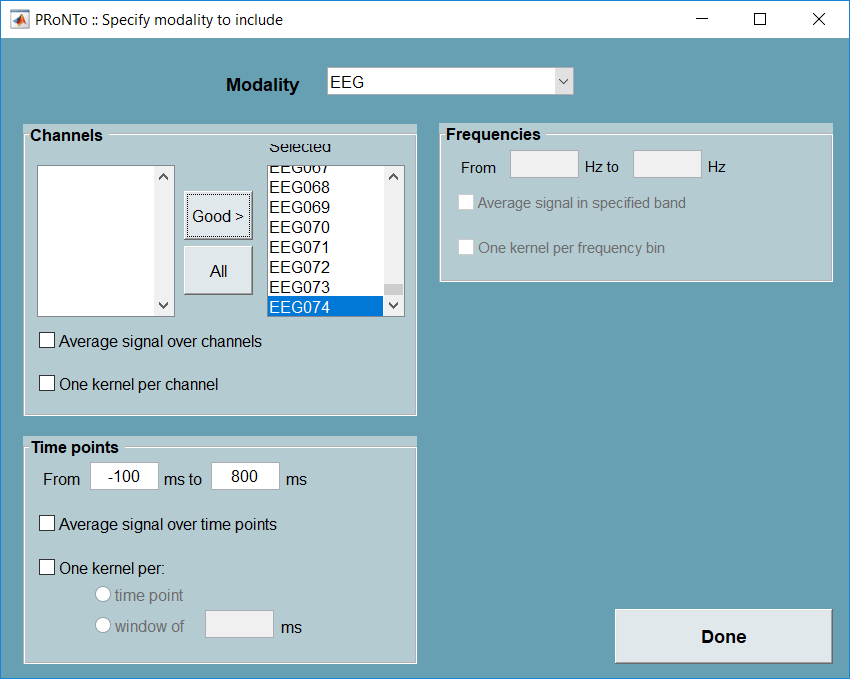
\includegraphics[scale=0.6]{images/Tutorial/v3/multimodal_face_tutorial/multimodal_face_gui_prepare_featureSet_specify_modality_meeg.png}
		  \captionsetup{width=0.9\linewidth}
	\captionof{figure}{`Specify modality' GUI for MEEG.}
	\label{fig:multimodal_face_gui_prepare_featureSet_specify_modality_meeg}
\end{minipage}%
	\begin{minipage}[b][9.5cm][b]{0.5\textwidth}
  \centering
		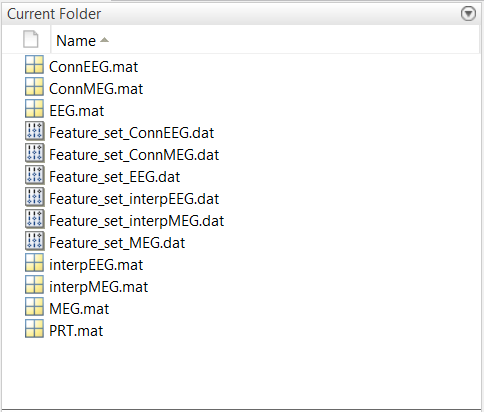
\includegraphics[scale=0.6]{images/Tutorial/v3/multimodal_face_tutorial/multimodal_face_gui_prepare_featureSet_final_files.png}
		\captionsetup{width=0.9\linewidth}
	\captionof{figure}{The files of the 6 feature sets.}
	\label{fig:multimodal_face_gui_prepare_featureSet_final_files}
	\end{minipage}
\end{figure}

%------------------------------------------------------------------

\subsection{Model: Specify new}

Our goal is now to discriminate between the brain signals recorded during visualization of `Famous' faces and `Scrambled' faces. We will first build one model for each modality separately, to see how they perform, then we'll build a model that combines all the information and look at the contribution of each modality to the predictive model. By the end of this tutorial we are going to have a total of 8 different models, 6 single kernel models (one for each modality), one multiple kernel model, and a single kernel model using a 2nd level atlas only for demonstration purposes.


\begin{itemize}
	
	\item In PRoNTo's main window, click on `Specify model' and a new window called `Specify model' will open (see Figure \ref{fig:gui_specify_new} in Chapter \ref{sec:Block_design_fMRI_dataset}).
	
	\item Select the `PRT.mat' file and provide a meaningful name to the first model, e.g. `interpEEG\_SVM'.

	\item Select the `interpEEG' feature set previously defined.

	\item Leave the option `Use kernels' tick box as it is, i.e. `Yes'.

	\item	Select the `Classification' model type and click on the 'Define classes` button. A new window will open, `Specify classes', to define the number of classes and a name for each class. We will define 2 classes. First click `Class 1' on the tab `Class'. For `Class 1' select all subjects and the condition `Famous' and, similarly, for `Class 2' select all subjects and the condition `Scrambled'. A novelty in the class specification is the possibility to randomly subsample the over-represented class (to match as close as possible the under-represented class). However, we use only one condition per class and one image per subject, so our dataset is balanced. So leave the `Subsample according to smallest class' unchecked. Once you have appropriately specified everything, click `Done'.
	
	\item Select the `Binary support vector machine' option, in the `Machine' field.
	
	\item Select the `Optimize hyper-parameter' tick box, in the `Define Range' put `[0.1 1 10 100]' and in the `Cross-Validation Scheme' (internal loop) field, select the option `k-fold CV on Subject out'. A window will appear asking to define the value of k, set it to 4.
		
	\item Select the same cross-validation scheme for the external loop as well.
	
\textbf{Note:} ‘Leave One Subject per Class Out’ or its k-folds variant is not appropriate here as we need to leave out all images from a single subject. Using the `per Class Out' CV will throw an error and ask to select ‘Leave Subject Out’ instead.
	
	\item In the `Data operations' box, select the `Mean centre features using training data' option.
	
In the end, the `Specify model new' window should look similar to the one in figure \ref{fig:multimodal_face_gui_specify_model_new_final}.
	
	\item Permutation testing is set in the `Run model' module and since we are going to run permutations, we are only going to specify the model here, and run it later. So click on `Specify model'.

\end{itemize}

This operation could be repeated across the different modalities. However, this is tiresome and prone to human errors. In addition, if we had used the subsampling option, the different models would very likely select different samples, which would make them harder to compare. Instead, we can now copy most of the parameters from the model we just defined. This is done in the next section using the `Specify model from' module.

\subsection{Model: Specify from}

The main interface has been modified to add a `Specify from' model option. This will launch a window that is very similar to the `Specify model' window, but with a couple of changes: there is an extra popup menu that allows to select which model to copy from. Some fields have also been disabled to ensure comparability of the models: only the feature sets, the machine (with its hyper-parameter optimization) and the operations can be modified. Classes/Regression selection and outer CV options cannot be modified.

\begin{itemize}
\item To create the other models based on each modality, we simply need to load our PRT and select the ‘interpEEG\_SVM’ model to copy from (it is by default the 1st model in the PRT).

\item We need to specify a model name for this new model, e.g. `interpMEG\_SVM'.

\item In the present case, we only want to change which feature set is used, so we click on `interpEEG' to deselect it and then click on the modality we would like to add, namely `interpMEG'.

\item In the `Data operations' select the `Mean centre features using training data' option.

\item Leave all the other parameters intact.

The `Specify model from' window should look similar to the one in figure \ref{fig:multimodal_face_gui_specify_model_from_final}.

\begin{figure}[!h]
	\centering
	\begin{minipage}[b][12.6cm][b]{0.5\textwidth}
  \centering
		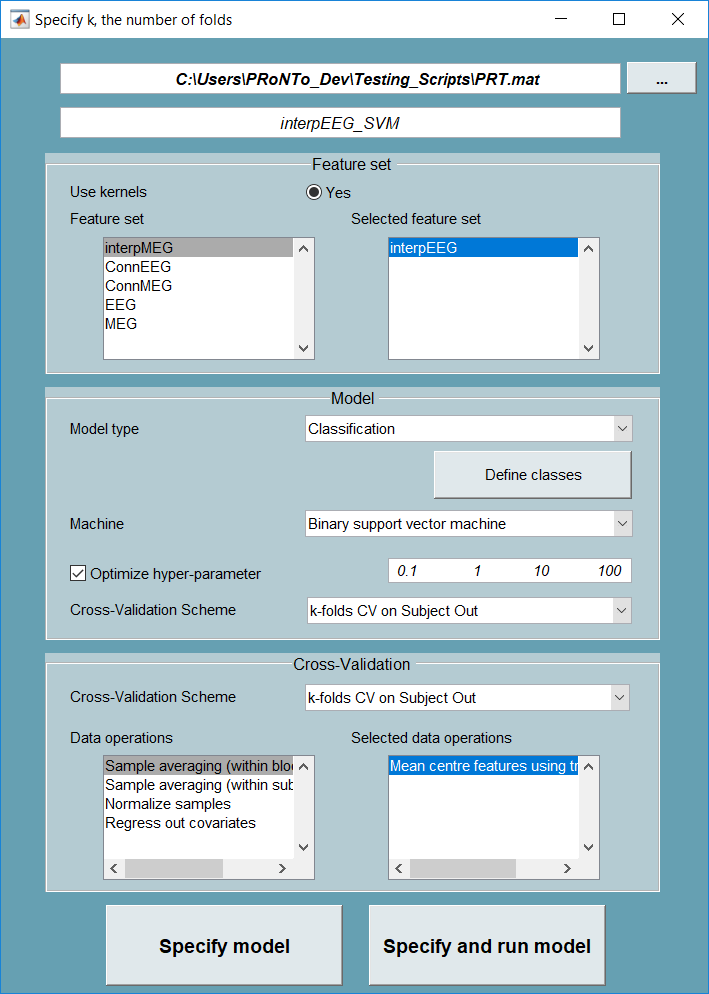
\includegraphics[scale=0.555]{images/Tutorial/v3/multimodal_face_tutorial/multimodal_face_gui_specify_model_new_final.png}
		  \captionsetup{width=0.7\linewidth}
	\captionof{figure}{`Model: Specify new' GUI final configuration.}
	\label{fig:multimodal_face_gui_specify_model_new_final}
\end{minipage}%
	\begin{minipage}[b][12.6cm][b]{0.5\textwidth}
  \centering
		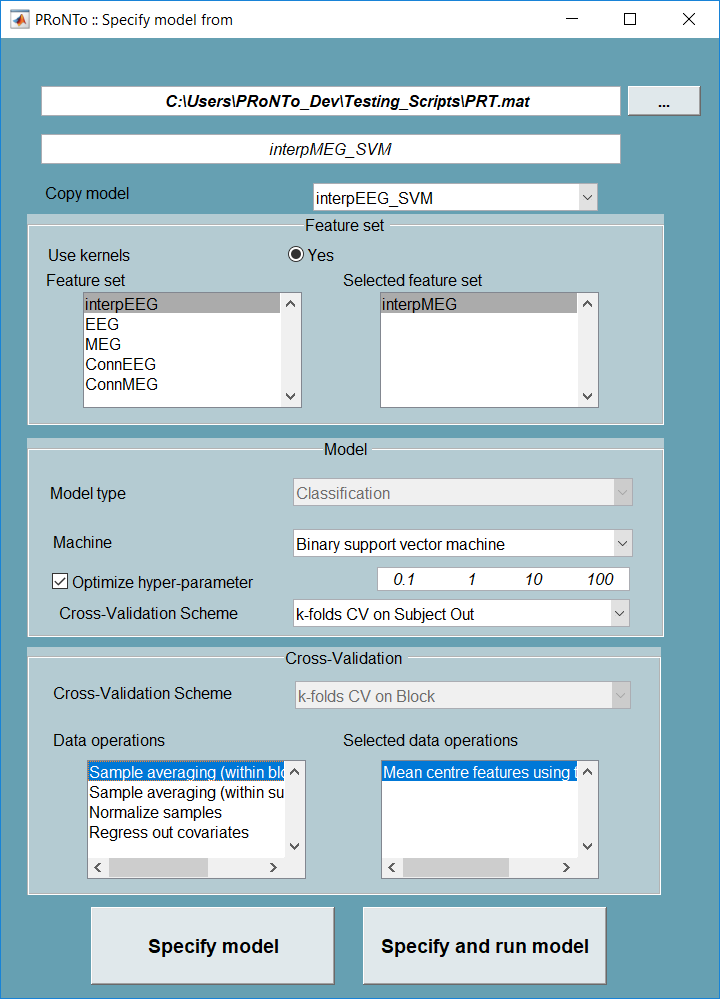
\includegraphics[scale=0.555]{images/Tutorial/v3/multimodal_face_tutorial/multimodal_face_gui_specify_model_from_final.png}
		\captionsetup{width=0.7\linewidth}
	\captionof{figure}{`Model: Specify from' GUI final configuration.}
	\label{fig:multimodal_face_gui_specify_model_from_final}
	\end{minipage}
\end{figure}

\item Do exactly the same procedure for the 4 other modalities, where each time you will only select the feature set of that modality with a name exactly the same as the feature set itself, adding a `\_SVM' in the end, e.g. `EEG\_SVM', `MEG\_SVM', `ConnEEG\_SVM', `ConnMEG\_SVM'.

\end{itemize}

\noindent \textbf{Understanding the `PRT' structure:} Now if you load and explore the `PRT.mat' file in the \matlab{} Workspace, you are going to see that there are some new structures, which correspond to the feature sets and the models you created. If you open the `PRT.model' you will see it has 3 fields, with 6 entries. The first one, `model\_name', you will recognize as the name of the model you wrote. Then we have the `input', which is the different parameters of the model, some of which you input manually and others that were defined automatically. Finally there is the `output', which is where the results of each model will be written once you run the models. At the moment it is empty since you haven't run the models yet.
\\

If for example you want to do a quick check of the feature set that you input in a model you want to build, one way through the \matlab{} Workspace is to get inside the `PRT.model' and go to the input of the first entry, `interpEEG\_SVM'. So now we ought to be inside `PRT.model(1).input' if you followed the instructions properly. Inside there, you will find a field named `fs'. `fs' in general is short for `feature set', and in that particular case corresponds to the feature set of this particular model. So if you followed the instructions properly, the feature set ought to be the `interpEEG'. It is in that particular structure that you will find more than one feature sets, corresponding to the feature sets, in the case of multiple kernel learning.
\\

\noindent \textbf{\underline{MKL model}}
\\

We can also build multimodal models in PRoNTo and use it to investigate the different contribution of each modality for the predictive model. In this example we can use the MKL model to investigate which modality contains most information for the `Faces' versus `Scrambled' comparison, and see if using different features improves performance when compared to the single modalities. So use the `Specify model from' module again, but this time instead of having only one feature set, add all feature sets to the model. You will also need to change the machine to the `L1 Multi-Kernel Learning'. Finally you will also need to add the `Normalize samples' operation in the `Data operations' to compensate for the fact that different modalities have different numbers of features. Leave all the other options as they are. The `Specify model from' window for the MKL model should look similar to the one in figure \ref{fig:multimodal_face_gui_specify_model_from_mkl_final}.

%------------------------------------------------------------------

\subsection{Model: Run}

We can use the `Run' module to run the previously specified models. After you select the `PRT.mat' file you will see the 7 models we have created so far, 6 single kernel models and the MKL model. You can either select and run them one by one, or you can select all and run them all together.
\\

In `Permutations' select `Perform permutation test' with 100 repetitions. Be aware that 100 repetitions is a small number when running permutation tests, and 1000 repetitions (or even more) are recommended if you want to be able to obtain smaller p-values (since the minimum p-value possible is equal to 1/number of permutations). The `Run' window should look similar to the one in figure \ref{fig:multimodal_face_gui_run_final}.

\begin{figure}[!h]
	\centering
	\begin{minipage}[b][13cm][b]{0.5\textwidth}
  \centering
		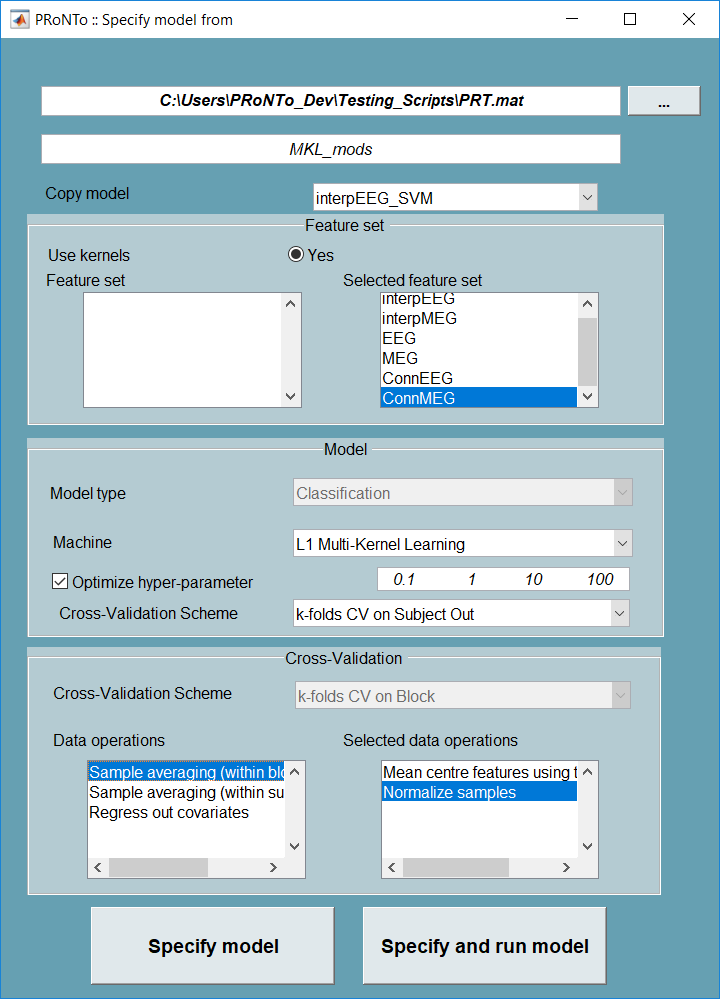
\includegraphics[scale=0.555]{images/Tutorial/v3/multimodal_face_tutorial/multimodal_face_gui_specify_model_from_mkl_final.png}
		  \captionsetup{width=0.8\linewidth}
	\captionof{figure}{`Model: Specify from' GUI final configuration for the MKL model.}
	\label{fig:multimodal_face_gui_specify_model_from_mkl_final}
\end{minipage}%
	\begin{minipage}[b][13cm][b]{0.5\textwidth}
  \centering
		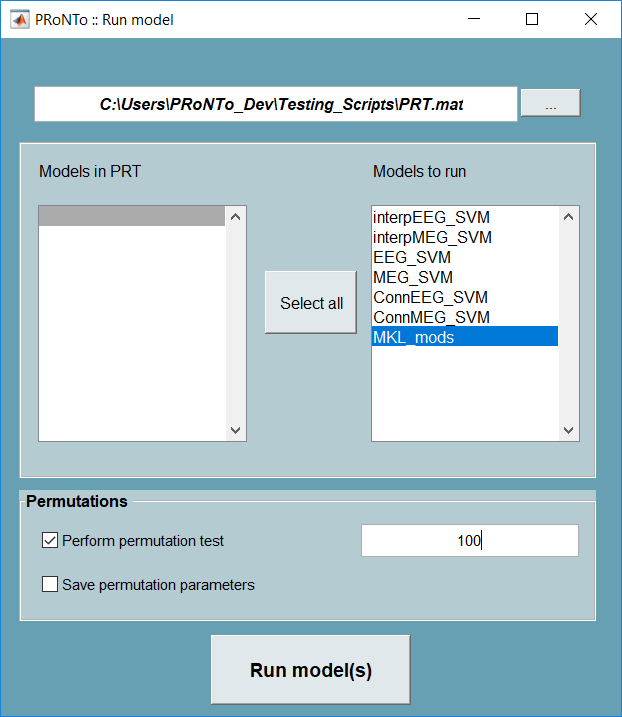
\includegraphics[scale=0.555]{images/Tutorial/v3/multimodal_face_tutorial/multimodal_face_gui_run_final.png}
		\captionsetup{width=0.8\linewidth}
	\captionof{figure}{`Model: Run' GUI final configuration to run all models together.}
	\label{fig:multimodal_face_gui_run_final}
	\end{minipage}
\end{figure}

%------------------------------------------------------------------

\subsection{Display results}

Taking a quick look at the results we see that `interpMEG\_SVM' and `MEG\_SVM' are the best performing models, and `ConnMEG\_SVM' the worst performing model. We also see that the MKL model that included all modalities had in fact worse performance than the best single-kernel modalities alone.
\\

For more detailed information regarding the interpretation of the results, the different types of ways to measure performance and the stats of the results the reader should take a look at all the previous tutorials, especially chapters \ref{sec:Block_design_fMRI_dataset} and \ref{data_example3}.

%------------------------------------------------------------------

\subsection{Compute weights}

Accordingly, the weight computation window includes a tick box to allow building the average weights for each permutation. As in the v2.X batch, these are saved in another folder. The window will also allow to select one atlas per feature set included in the model. To this end, simply select multiple images or .mat, in the correct order. If the ‘Computer average/kernel weight per region’ option is selected, feature sets that were built using an atlas will automatically use this atlas. If this option is selected and no atlas is specified for some feature sets, only the weights will be built, not the weights per region/kernel. Please note that loading an atlas for weight summarization is not available for MEEG data (only nifti and .mat).

\begin{itemize}

\item In PRoNTo's main window, click on `Compute weights' and a new window will open, `Compute weights' (Figure \ref{fig:gui_compute_weights}).

\item Select the `PRT.mat' file.

\item Select one by one all models from the list of `Models computed in PRT'.

% \item Check the option `Build weight images for permutations'. This is an \textbf{optional} step in case you want to do further statistical analyses with the weights later on.

\item Leave the options `Compute average/kernel weight per region' and `Build weight images for permutations' unchecked.

\item Click on `Compute weights' button. Computations will be displayed on the \matlab{} command window.

\end{itemize}

The final `Compute weights' window should look like the one in figure \ref{fig:multimodal_face_gui_compute_weights_final}

\begin{figure}[!h]
  \centering
		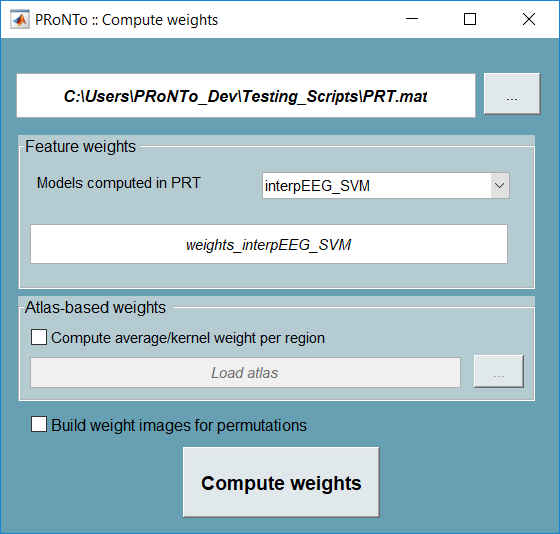
\includegraphics[scale=0.60]{images/Tutorial/v3/multimodal_face_tutorial/multimodal_face_gui_compute_weights_final.png}
	\caption{`Compute weights' GUI.}
	\label{fig:multimodal_face_gui_compute_weights_final}
\end{figure}

%------------------------------------------------------------------

\subsection{Display weights}

Weights can be displayed for all modality types. For 1D MEEG or 1D .mat data, weights are displayed as bar graphs, with the color of the bar representing the amplitude of the weight (e.g. the connectivity vector used for .mat). Example in figure \ref{fig:multimodal_face_gui_display_weights_1d}.

\begin{figure}[!h]
  \centering
		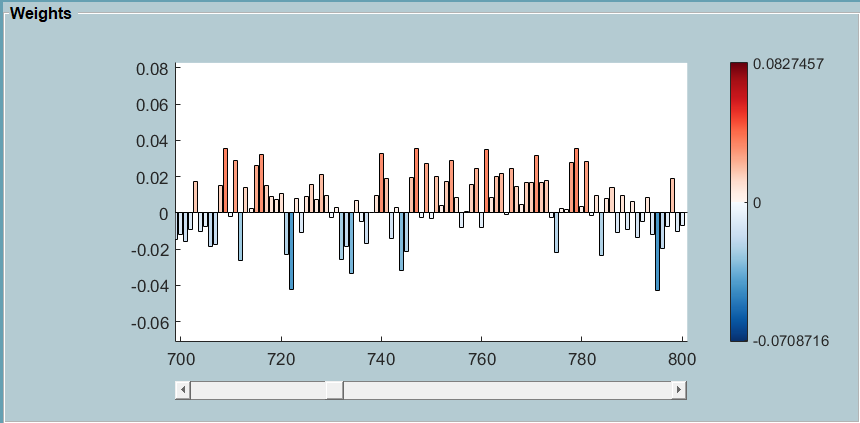
\includegraphics[scale=0.59]{images/Tutorial/v3/multimodal_face_tutorial/multimodal_face_gui_display_weights_1d.png}
	\caption{`Display weights' for 1D MEEG or .mat data.}
	\label{fig:multimodal_face_gui_display_weights_1d}
\end{figure}


\textbf{For 2D data}, the display shows the matrix, with y-axis as the 1st dimension and x-axis as the 2nd dimension (after squeezing out dimensions of size 1), with the color of a (x,y) pair displaying the magnitude of its weight. Example in figure \ref{fig:multimodal_face_gui_display_weights_2d}. Finally, nifti images are displayed as before, except a small change in the color map. Example in figure \ref{fig:multimodal_face_gui_display_weights_nifti}.


\begin{figure}[!h]
  \centering
		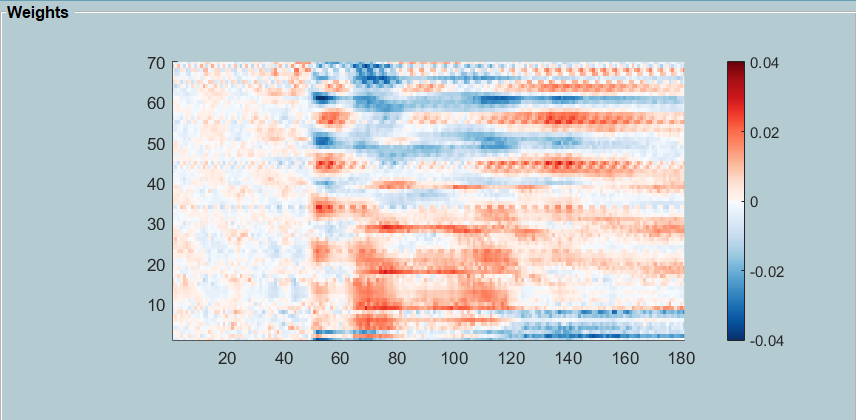
\includegraphics[scale=0.59]{images/Tutorial/v3/multimodal_face_tutorial/multimodal_face_gui_display_weights_2d.png}
	\caption{`Display weights' for 2D MEEG or .mat data.}
	\label{fig:multimodal_face_gui_display_weights_2d}
\end{figure}

\begin{figure}[!h]
  \centering
		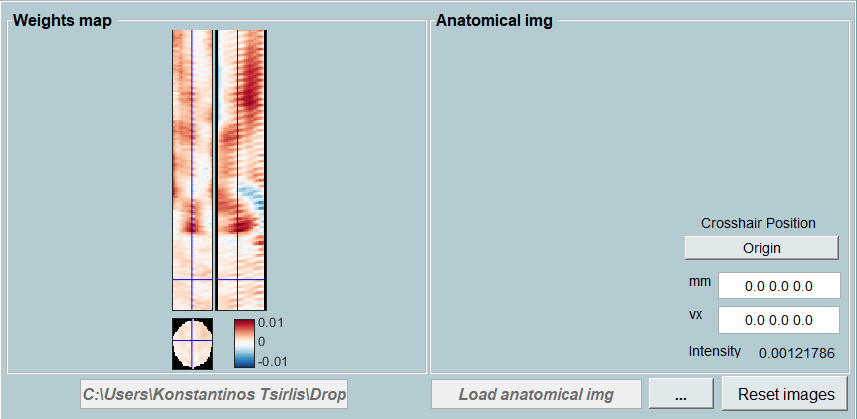
\includegraphics[scale=0.59]{images/Tutorial/v3/multimodal_face_tutorial/multimodal_face_gui_display_weights_nifti.png}
	\caption{`Display weights' for nifti images.}
	\label{fig:multimodal_face_gui_display_weights_nifti}
\end{figure}

When building the weights from the `MKL\_mods' model, we can also look at the feature set contributions. From figure \ref{fig:multimodal_face_gui_display_weights_mkl} we can see that the interpolated EEG has the largest contribution to the MKL model, followed by the EEG and MEG traces. This can be due to the interpolated EEG smoothing some of the anatomical variance in electrode placement, while EEG and MEG keep subject-specific information.

\begin{figure}[!h]
  \centering
		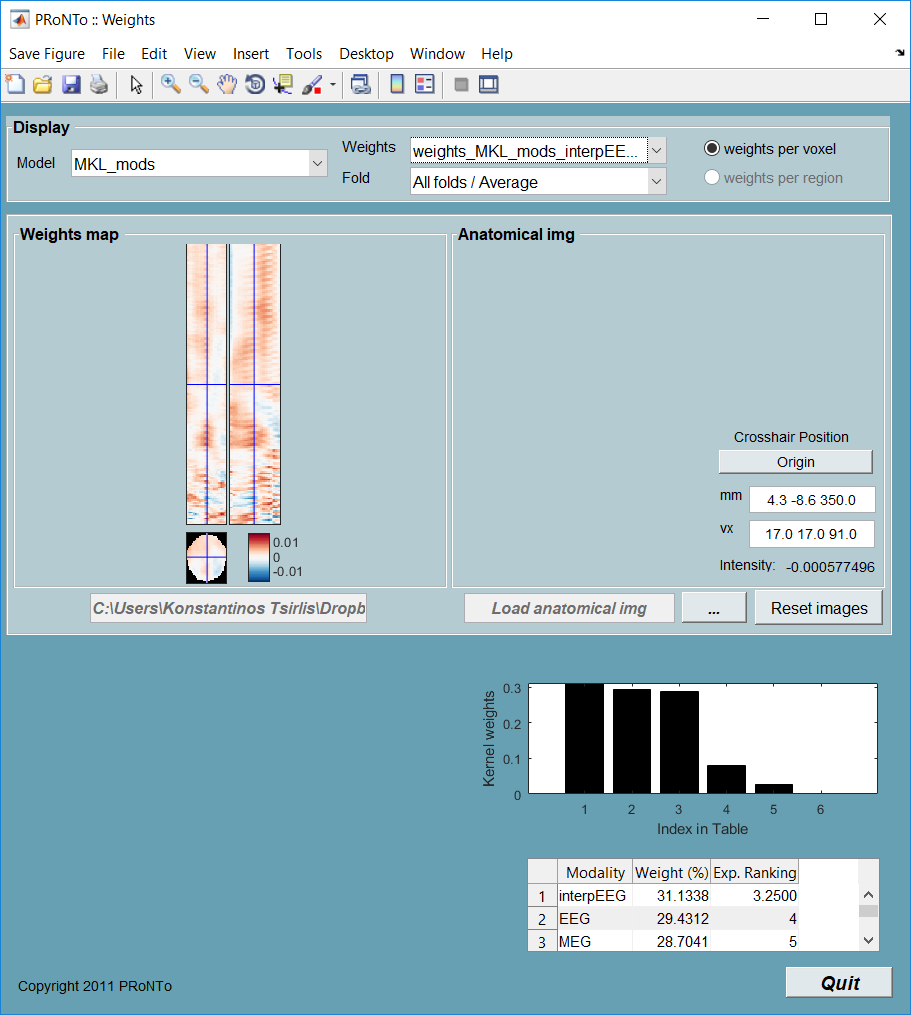
\includegraphics[scale=0.6]{images/Tutorial/v3/multimodal_face_tutorial/multimodal_face_gui_display_weights_mkl.png}
	\caption{`Display weights' for MKL model, with additional weight contribution shown.}
	\label{fig:multimodal_face_gui_display_weights_mkl}
\end{figure}

%------------------------------------------------------------------

\subsection{Using an atlas with .mat}
\label{ssec:atlas_w_mat}

As for nifti, an atlas can be used with .mat and MEEG files. For MEEG files, the atlas is implicit, resulting from the selection of channels, time points and kernels on which to build the kernels on. However, for .mat, PRoNTo is agnostic of the type of features entered, so the atlas needs to be built by the user. As an example, we built an atlas for the EEG connectivity derived modality. We defined 11 `networks' that the channels could belong to based on their anatomical position (e.g. `orbitofrontal', `occipital', `left-parietal', `central-parietal', ...). The atlas then builds ROIs from pair-wise network interactions (i.e. `orbitofrontal-occipital', `orbitofrontal – left-parietal', ...) leading to 66 ROIs (11*10/2 between networks interactions + 11 within-network interactions). The atlas looks as in figure \ref{fig:multimodal_face_Atlas_EEG_Conn_EEG} (2D version but only the upper triangular part is saved).
\\

\begin{figure}[!h]
  \centering
		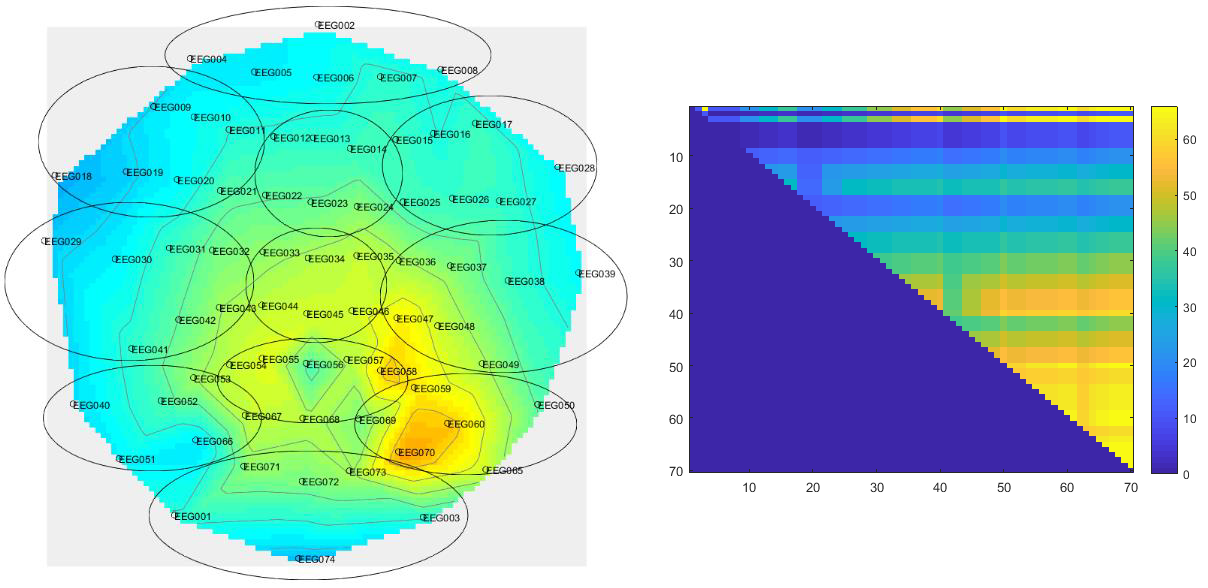
\includegraphics[scale=0.60]{images/Tutorial/v3/multimodal_face_tutorial/multimodal_face_Atlas_EEG_Conn_EEG.png}
	\caption{Atlas for EEG connectivity modality, defining interactions between and within 11 `networks' (identified based on their anatomical position as displayed on the left).}
	\label{fig:multimodal_face_Atlas_EEG_Conn_EEG}
\end{figure}

Going back to the feature set step, we can build another .mat feature set (called `ConnEEG\_atlas') including the ConnEEG modality and ticking the `Build one kernel per ROI' box (figure \ref{fig:multimodal_face_gui_prepare_featureSet_specify_modality_ConnEEG_atlas}. We can load the designed atlas and PRoNTo will automatically gather ROI labels if a label file (called `Labels\_\textit{atlasname}.mat') is present in the same folder and contains a `ROI\_names' variable.
\\

Model specification can then be performed as in v2.

\begin{itemize}
\item Select the `ConnEEG\_atlas' feature set.
\item Define the classes as we did before.
\item Choose the `L1 Multi-Kernel Learning' machine. 
\item Use 4-folds CV on subjects out for both inner and outer CV.
\item And finally, add the mean centering and the normalize samples operations before specifying and running. 
\end{itemize}

The window should look like the one in figure \ref{fig:multimodal_face_gui_specify_model_ConnEEG_atlas_MKL}.
\\

\begin{figure}[!h]
	\centering
	\begin{minipage}[b][13cm][b]{0.5\textwidth}
  \centering
		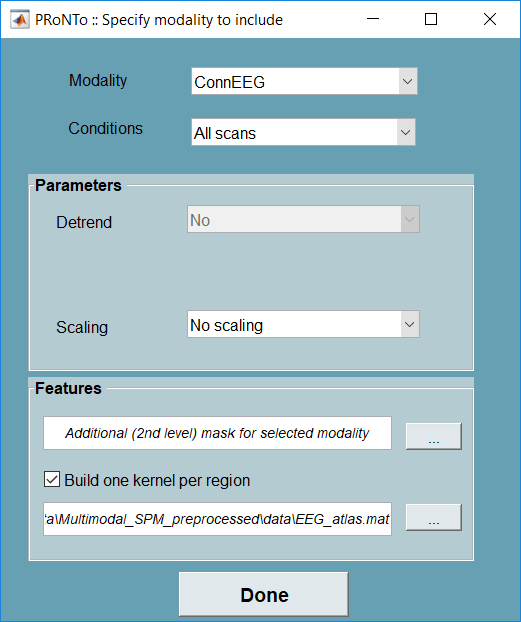
\includegraphics[scale=0.65]{images/Tutorial/v3/multimodal_face_tutorial/multimodal_face_gui_prepare_featureSet_specify_modality_ConnEEG_atlas.png}
		  \captionsetup{width=0.9\linewidth}
	\captionof{figure}{`Specify modality' GUI with atlas.}
	\label{fig:multimodal_face_gui_prepare_featureSet_specify_modality_ConnEEG_atlas}
\end{minipage}%
	\begin{minipage}[b][13cm][b]{0.5\textwidth}
  \centering
		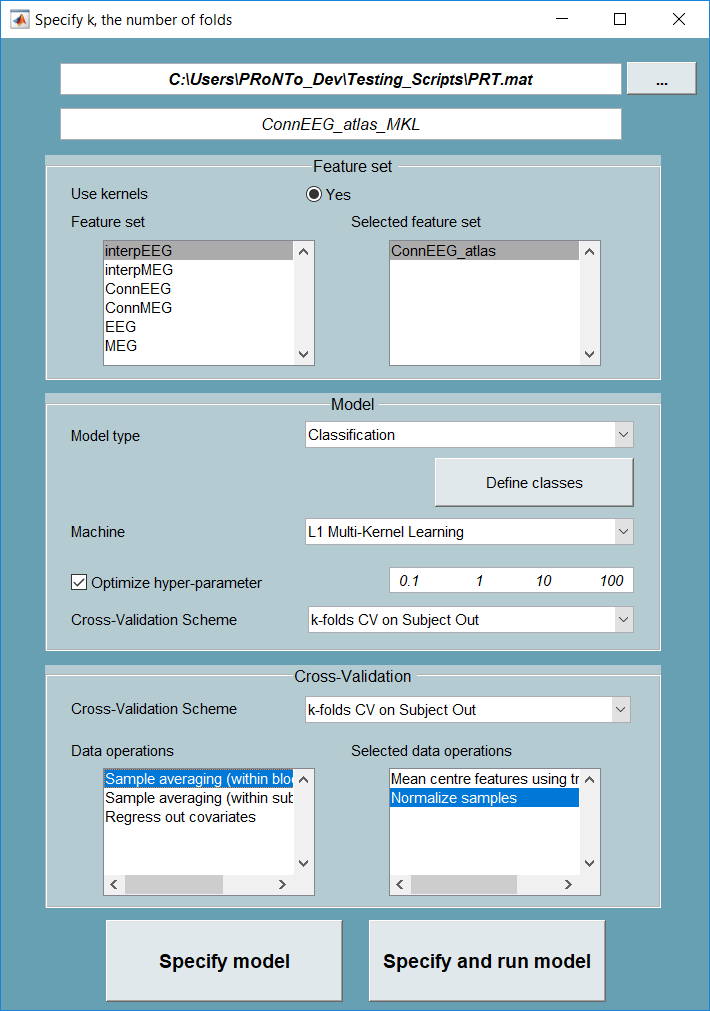
\includegraphics[scale=0.5]{images/Tutorial/v3/multimodal_face_tutorial/multimodal_face_gui_specify_model_ConnEEG_atlas_MKL.png}
		\captionsetup{width=1\linewidth}
	\captionof{figure}{`Specify model' GUI final configuration.}
	\label{fig:multimodal_face_gui_specify_model_ConnEEG_atlas_MKL}
	\end{minipage}
\end{figure}


The model does not perform very well (53.13\% balanced accuracy) for this modality taken on its own. For information, the same model using SVM (i.e. discarding the atlas information) leads to 43.75\% balanced accuracy. Both models display a large variance across folds and would not be considered as significantly discriminating between famous faces and scrambled faces.
\\

We can compute the weights for this model and select the option to build the weights per region. This will build 2 .mat files: one including the weights per feature, one including the weights per ROI. The latter gives the same value (i.e. its kernel contribution) to each feature within a ROI. The `Display weights' window in figure \ref{fig:multimodal_face_gui_display_weights_per_region} shows the table of kernel contributions.
\\

\textbf{Note:} If for any reason the ROI labels haven't loaded, you can manually load them using the button `Load labels' and locating the file `Labels\_EEG\_atlas.mat' found in $Multimodal\_face\_dataset/data$.

\begin{figure}[!h]
  \centering
		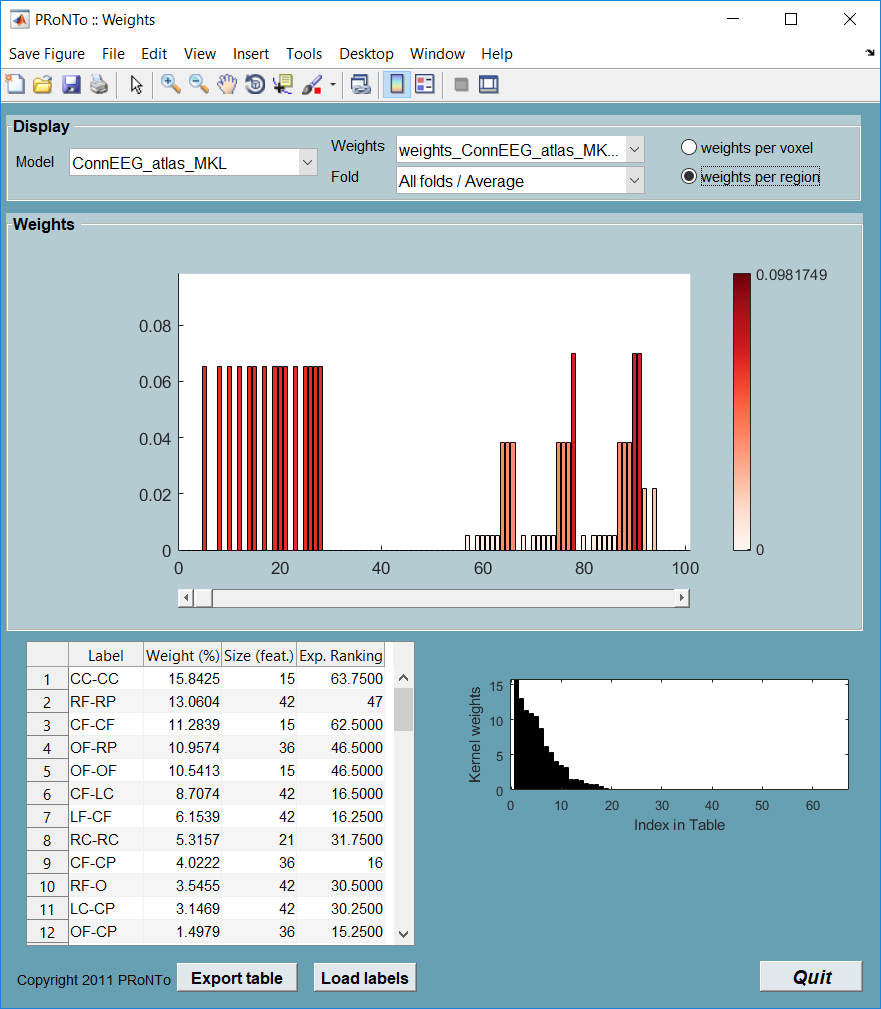
\includegraphics[scale=0.5]{images/Tutorial/v3/multimodal_face_tutorial/multimodal_face_gui_display_weights_per_region.png}
	\caption{Atlas for EEG connectivity modality, defining interactions between and within 11 `networks' (identified based on their anatomical position as displayed on the left).}
	\label{fig:multimodal_face_gui_display_weights_per_region}
\end{figure}

The weight file can then be postprocessed for better visualization. This has to be performed outside of PRoNTo as PRoNTo does not know what type of data the .mat represents (i.e. it does not know this is connectivity data).
\\

As an example, in figure \ref{fig:multimodal_face_summarized_ROI_weights_Conn_EEG_and_schemaball} we have summarized the weights per region in a 11*11 matrix instead of the 70*70 matrix. Furthermore, a schemaball plot (code modified from \matlab{}’s file exchange schemaball submission, in appendix) was derived. It depicts the contribution of each between-network interaction to the classification as a colored curve and the within-network contributions as node color and size.
\\
\vfill

\begin{figure}[!h]
  \centering
		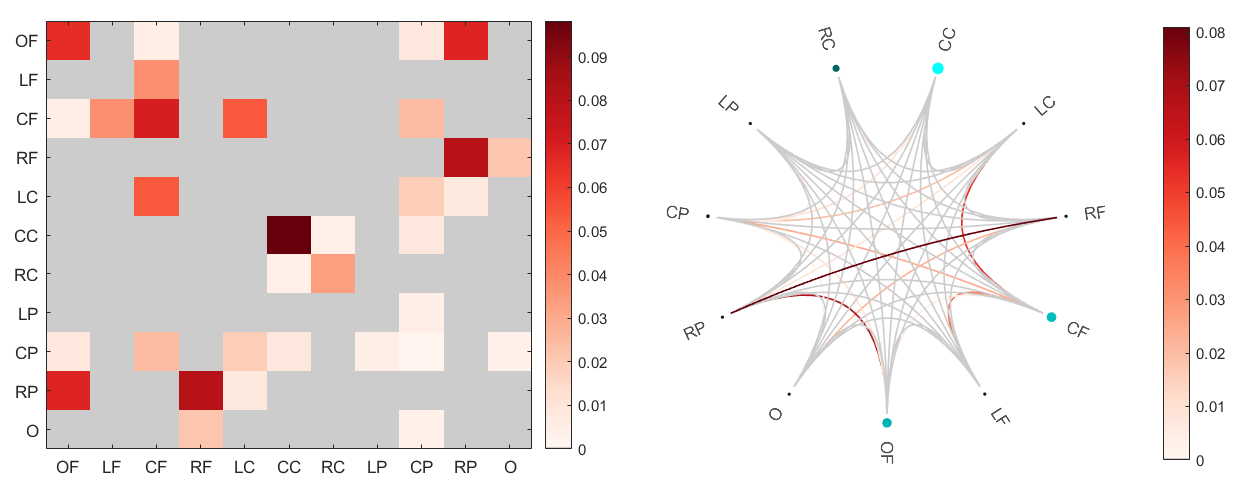
\includegraphics[scale=0.5]{images/Tutorial/v3/multimodal_face_tutorial/multimodal_face_summarized_ROI_weights_Conn_EEG_and_schemaball.png}
	\caption{Summarized ROI weights across networks, displayed as a matrix (left) and as a schemaball (right). The size and brightness of the network marker displays the within-network contribution while the curves display the between-network contributions. Grey lines or matrix entries represent 0 contribution.}
	\label{fig:multimodal_face_summarized_ROI_weights_Conn_EEG_and_schemaball}
\end{figure}


%------------------------------------------------------------------

\section{Batch analysis}

This tutorial will now show how to analyse the same data but using the {\tt matlabbatch} system.
\\

Once again, to analyse the data, create a new directory in which to save the results of the analysis, saved as 'PRT.mat'. On the main interface of PRoNTo click on the 'Batch' button to open the `{\tt matlabbatch}'. Alternatively, type `prt\_batch' in the \matlab{} prompt.

\subsection{Data \& Design}

When adding a modality, the user now has to specify its ‘Data format’ as either nifti, MEEG or .mat. As the batch is agnostic of the user’s choices, all design options are available for each type. Please make sure to use the appropriate option (i.e. loading an SPM.mat is only for nifti, and ‘Events in file’ is only for MEEG).
\\

For the same reason, one mask has to be entered per modality, independent of its type. Only `nifti' data format requires a file, `.mat' and `MEEG' just need a modality name. This is in contrast with the GUI that only requires masks for `nifti' files (as it derives the masks for the MEEG and .mat automatically).

\begin{itemize}

	\item Click on `Data \& Design' in the PRoNTo `{\tt matlabbatch}' menu.

	\item In the `Directory' field, select a directory where the `PRT.mat' file will be saved.
	
	\item In the `Groups' field:
 	
		\begin{itemize}
		
		\item Add one group and in the field `Name', provide a name without spaces to that group, e.g. `G1'. 
		
		\item In the field `Select by', select the `Subjects' option and add one subject.
		\end{itemize}
		
		\begin{itemize}
		    \item []
		\textbf{\underline{EEG/MEG (MEEG data format)}}
		\begin{itemize}
        
		\item Add one modality for this subject and provide a name, e.g. `EEG'; choose the appropriate data format (here MEEG); define the interscan interval of 0.05 seconds; and in the field `Files', select the EEG (MEEG) file of the first subject (`S1'), found in the $Multimodal\_face\_dataset/data/S1$ directory.
		
		\item In the `Data \& Design' field, since our data are in MEEG format, choose the `Events in MEEG file' (for MEEG inputs only option), and select no regression targets/covariates.
		
		\item Add one more modality and repeat the whole procedure for MEG.
		\end{itemize}
		
		\textbf{\underline{Connectivity EEG/MEG (.mat data format)}}
		\begin{itemize}

		\item Add two more modalities, these would be the `ConnEEG' and `ConnMEG'; choose the appropriate data format (here .mat); define the interscan interval at 1; and in the field `Files', select the 3 ConnEEG/ConnMEG (.mat) files of the first subject (`S1'), found in the $Multimodal\_face\_dataset/data/S1$ directory. Remember that the order (Unfamiliar, Famous, Scrambled) with which you input the files is of great importance.
		
		\item In the `Data \& Design' field, since our data are in .mat format, choose the `Specify design' option, set the `Units for design' to `Scans', and either manually set the names, onsets and durations of each of the 3 conditions, or select the practical option `Multiple conditions' and select the `Design.mat' file found in the $Multimodal\_face\_dataset/data/S1$ directory.
		
		\item Repeat the whole procedure for MEG.

		\end{itemize}
		
        \textbf{\underline{Interpolated EEG/MEG (nifti data format)}}
		\begin{itemize}

		\item Add two more modalities, these would be the `interpEEG' and `interpMEG'; choose the appropriate data format (here nifti); define the interscan interval at 1; and in the field `Files', select the 3 interpEEG/interpMEG (NIfTI) files of the first subject (`S1'), found in the $Multimodal\_face\_dataset/data/S1$ directory in the folders $EEG\_interp/MEG\_interp$. Remember that the order (Unfamiliar, Famous, Scrambled) with which you input the files is of great importance.
		
		\item In the `Data \& Design' field, since our data are in .mat format, choose the `Specify design' option, set the `Units for design' to `Scans', and either manually set the names, onsets and durations of each of the 3 conditions, or select the practical option `Multiple conditions' and select the `Design.mat' file found in the $Multimodal\_face\_dataset/data/$ directory.
		
		\item Repeat the whole procedure for MEG.

		\end{itemize}
		
		\end{itemize}

    \item In the `Masks' field, add 6 new modalities and provide the appropriate modality names. The name of the modality here has to be exactly the same as in `Modalities', otherwise it will not work.
    
    \begin{itemize}
    \item For MEEG and .mat you only have to choose the appropriate data format as for both of these data formats we assume that the users have provided only useful features, as this can be easily performed during pre-processing. Please ensure that your data do not contain NaNs.
    
    \item For nifti select the `mask\_EEG' or the `mask\_MEG' masks found in the $Multimodal\_face\_dataset/data/$ directory and ensure that `HRF overlap' and the `HRF delay' fields are 0.
    \end{itemize}

\item In the `Review' field, select `Yes' if you would like to review your data and design in a separate window. Otherwise, leave as it is, i.e. `No'. Keep in mind that the procedure pauses while you review the data and that you have to close the `Review' window for the procedure to continue.

\end{itemize}

\begin{figure}[!h]
  \centering
		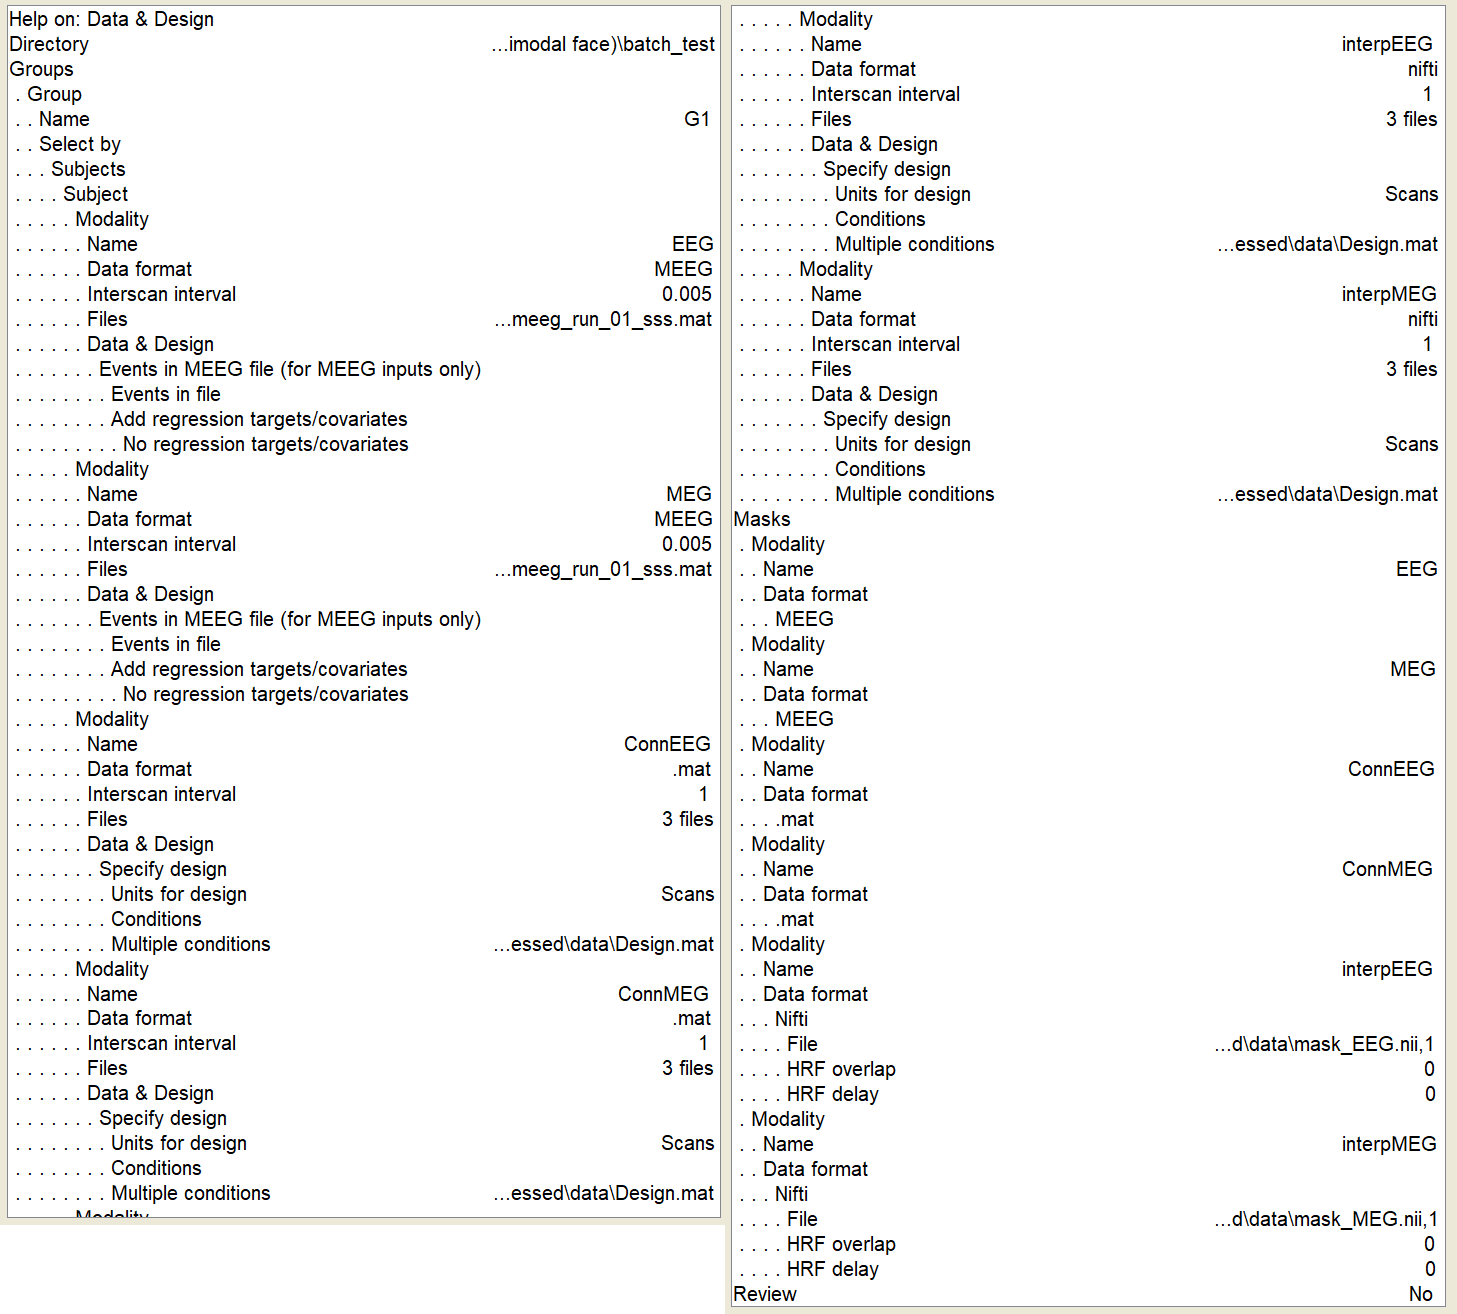
\includegraphics[scale=0.4]{images/Tutorial/v3/multimodal_face_tutorial/multimodal_face_batch_data_and_design_final.png}
	\caption{`Data \& Design' module in {\tt matlabbatch}.}
	\label{fig:multimodal_face_batch_data_and_design_final}
\end{figure}

After you have set everything for the first subject, you can go to `Subjects' and select `Replicate: Subject (1)'. That way you will have everything set and you will only need to change the files from those of `S1' to the ones of the subject you are setting. Alternatively, you could use the `PRT.mat' you already have from the GUI part of the tutorial, or use the script we provide. The final configuration including the first subject only should look like figure \ref{fig:multimodal_face_batch_data_and_design_final}.
\vfill

%------------------------------------------------------------------

\subsection{Feature set / Kernel}


\textbf{\underline{Interpolated EEG/MEG (nifti data format)}}
\begin{itemize}
	\item Click on `Feature set / Kernel' option on PRoNTo's {\tt matlabbatch} menu.
	
	\item With `Load PRT.mat' field selected, click on the `Dependency' button to associate the `PRT.mat' file created in the previous `Data \& Design' step or click on the `Select files' button to browse where `PRT.mat' file was saved. The window of Figure \ref{fig:batch_feature_set_dep} in Chapter \ref{sec:Block_design_fMRI_dataset} is called to establish a dependency connection with the previous `Data \& design' module.

	\item Provide a name to the `Feature/kernel' set, e.g. `interpEEG'.
	
	\item Select the `Nifti' option for a data format, add one modality and select the modality name with the `Dependency' button or type it in manually but the name needs to be {\it exactly} the same as the one specified in the `Data \& Design' module, here `interpEEG'.
	
	\item Leave all the other parameters at their default options/values.
	
	\item Click on `Feature set / Kernel' option on PRoNTo's {\tt matlabbatch} menu to add one more `Feature set / Kernel' module and repeat the procedure for the interpolated MEG (`interpMEG') data.
	
	\end{itemize}	

	
\noindent \textbf{\underline{EEG/MEG (MEEG data format)}}
\begin{itemize}
    \item Click on `Feature set / Kernel' option on PRoNTo's {\tt matlabbatch} menu.
	
	\item With `Load PRT.mat' field selected, click on the `Dependency' button to associate the `PRT.mat' file created in the previous step or click on the `Select files' button to browse where `PRT.mat' file was saved.

	\item Provide a name to the `Feature/kernel' set, e.g. `EEG'.
	
	\item Select the `MEEG' option for a data format, add one modality and select the modality name with the `Dependency' button or type it in manually but the name needs to be {\it exactly} the same as the one specified in the `Data \& Design' module, here `EEG'.
	
	\item Leave all the other parameters at their default options/values.
	
	\item Click on `Feature set / Kernel' option on PRoNTo's {\tt matlabbatch} menu to add one more `Feature set / Kernel' module and repeat the procedure for the MEG (`MEG') data.

	\end{itemize}
	

\noindent \textbf{\underline{Connectivity EEG/MEG (.mat data format)}}
\begin{itemize}
    \item Click on `Feature set / Kernel' option on PRoNTo's {\tt matlabbatch} menu.
	
	\item With `Load PRT.mat' field selected, click on the `Dependency' button to associate the `PRT.mat' file created in the previous step or click on the `Select files' button to browse where `PRT.mat' file was saved.

	\item Provide a name to the `Feature/kernel' set, e.g. `ConnEEG'.
	
	\item Select the `.mat' option for a data format, add one modality and select the modality name with the `Dependency' button or type it in manually but the name needs to be {\it exactly} the same as the one specified in the `Data \& Design' module, here `ConnEEG'.
	
	\item Leave all the other parameters at their default options/values.
	
	\item Click on `Feature set / Kernel' option on PRoNTo's {\tt matlabbatch} menu to add one more `Feature set / Kernel' module and repeat the procedure for the connectivity MEG (`ConnMEG') data.

	\end{itemize}

 \noindent At this point your {\tt matlabbatch} should look like figure \ref{fig:multimodal_face_batch_prepare_featureSet_final}.
	
	\begin{figure}[!h]
	\centering
		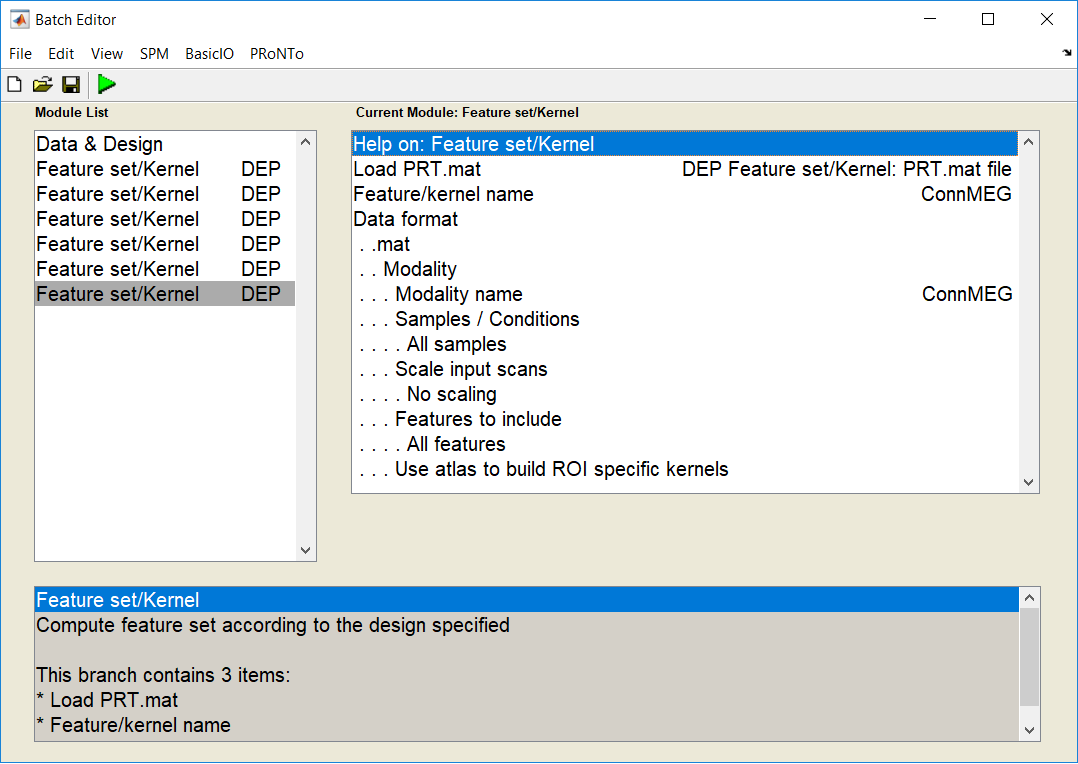
\includegraphics[width=0.6\textwidth]{images/Tutorial/v3/multimodal_face_tutorial/multimodal_face_batch_prepare_featureSet_final.png}
	\caption{`Feature set / Kernel' module in {\tt matlabbatch}.}
	\label{fig:multimodal_face_batch_prepare_featureSet_final}
\end{figure}

%------------------------------------------------------------------

\subsection{Model: Specify new}

\textbf{\underline{Single kernel models}}

\begin{itemize}

\item Click on the `Model: Specify new' option on PRoNTo's {\tt matlabbatch} menu.
	
	\item With `Load PRT.mat' field selected, click on the `Dependency' button to associate the `PRT.mat' file created in the previous `Feature set / Kernel' step or click on the `Select files' button to browse where `PRT.mat' file was saved.
	
	\item In the `Feature sets' field, select the `New: Name' in the `Feature set name' and either use the `Dependency' button to find the relevant feature set name (here `interpEEG\_SVM') or write it {\it exactly} as previously defined in its relevant `Feature set / Kernel' module.

	\item Select the `Classification' model type:
	
		\begin{itemize}
		
		\item Add 2 new classes.
		
		\item For Class (1) write `Famous' on the name field and add one group. Select the group name from the `Data \& Design' module (`Data \& Design:Group\#1 name') with the `Dependency' button, or write it {\it exactly}, as previously defined in the Data \& Design' module, here `G1'. Similarly, for Class (2) write `Scrambled' on the name field and add the group created in the `Data \& Design' module, `G1'.	
		
		\item In the `Subjects' field, type `1:16' to include all 16 subjects.
		
		\item In the `Conditions / Scans' field, select the `Specify Conditions' option and add a new condition in each class. Provide a name for this condition, i.e. for Class (1) `Famous' and for Class (2) `Scrambled'. Note that this name needs to be spelled exactly as specified in the `Data \& Design' module.
		
		\end{itemize}

        \item Leave `Subsample examples based on class definition' as it is, i.e. `No'.

	\item In the `Machine' field:
	
	\begin{itemize}
	
	\item Select the `Kernel machine' and the `SVM Classification' option.	
	
	\item In the `Machine optimization and parameters' field, select the `Optimize hyper-parameter' option.
	
	\item Set the `Regularization hyper-parameter' to `0.1, 1, 10, 100'.
	
	\item Set the `Cross-validation type for hyper-parameter optimization' to `k-folds CV on subjects' and the k to `4'. This is the internal cross-validation loop.
	
	\end{itemize}
	
	\item In the `Cross validation type' (external loop) field, select `k-folds CV on subjects' option and again set k to `4'.
	
	\item Leave the `Include all scans' field as it is, i.e. `No'.

	\item Leave all the rest to their default parameters/values.
	
% 		\begin{itemize}
% 		\item  Leave the `Mean centre features' field as it is, i.e. `Yes'. 
				
% 		\item  Click on the `Other Operations' field and select the option `Select Operations', then add a new operation and select the `Normalize samples' option.
% 		\end{itemize}
	
\end{itemize}

Figure \ref{fig:multimodal_face_batch_model_specify_new_final} shows the final configuration of the first {\tt matlabbatch} `Model: Specify new' module for the interpolated EEG data.
\\

	\begin{figure}[!h]
	\centering
		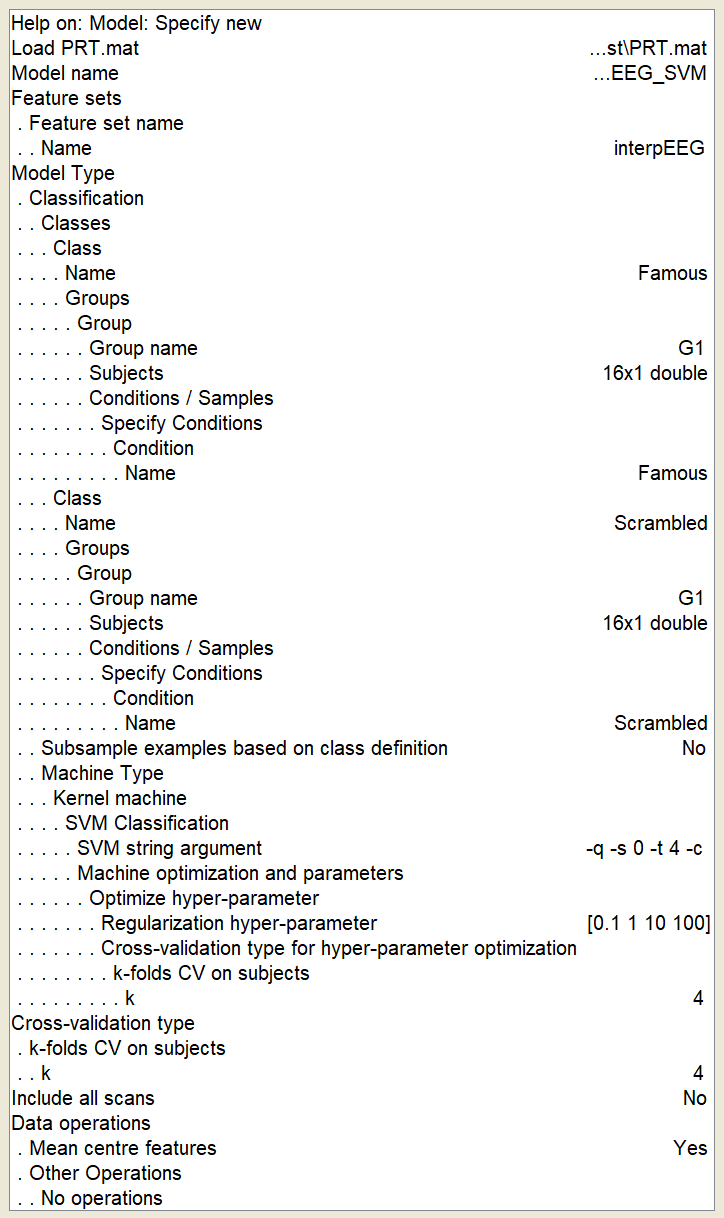
\includegraphics[scale=0.5]{images/Tutorial/v3/multimodal_face_tutorial/multimodal_face_batch_model_specify_new_final.png}
	\caption{Final configuration of the {\tt matlabbatch} `Model: Specify new' module.}
	\label{fig:multimodal_face_batch_model_specify_new_final}
\end{figure}

\noindent We now need to do the same procedure for 5 more single kernel models, each one including only 1 feature set, and for 1 multi-kernel model including all feature sets together.
\\

Compared to the GUI, when we are in {\tt matlabbatch} and depending on whether you want to modify the feature sets, the model types and the data operations from one model to the other, it might be more practical either to replicate the `Model: Specify new' module that we have already finished, or to create a new `Model: Specify from' module. In our case that we do not want to modify anything other than changing the feature set, it is in fact faster to just right-click on the `Model: Specify new' and select the `Replicate module' option.
\\

After replicating the finished module 5 times, for each module you will only need to change its `Model name' and the `Name' option of the `Feature set name' field. So for the other modules these would have to be interpMEG\_SVM' and `interpMEG' respectively, `EEG\_SVM' and `EEG', and so on.
\\

If one wanted to use the `Model: Specify from' module, then they would mostly have to follow the same procedure as in the `Model: Specify new' module, but they should also input the model they want to copy from in the `Model to copy' field, and also to specify in the `Fields to modify' any possible changes they wanted in either the feature sets, the model types or the data operations.
\\[3cm]

\noindent \textbf{\underline{Multi-kernel model}}

\begin{itemize}
    
    \item Replicate one `Model: Specify new' module one more time.
    
    \item Set a name for the model, `MKL\_mods'.
    
    \item We are going to include all 6 feature sets in this model, so in the `Feature set name' include 6 entries and put the 6 names of the feature sets, `interpEEG', `interpMEG', `EEG', `MEG', `ConnEEG' and `ConnMEG'.
    
    \item The second thing we will need to change is in the `Data operations' where in the `Other Operations' we are going to select the `Select Operations' option, include a new operation, and choose the `Normalize samples' option from the list.
    
    \item Leave all the other fields as they are.
    
\end{itemize}


Figure \ref{fig:multimodal_face_batch_model_specify_new_all} shows all 7 {\tt matlabbatch} `Model: Specify new' modules, with the MKL model showing as an example.

\begin{figure}[!h]
	\centering
		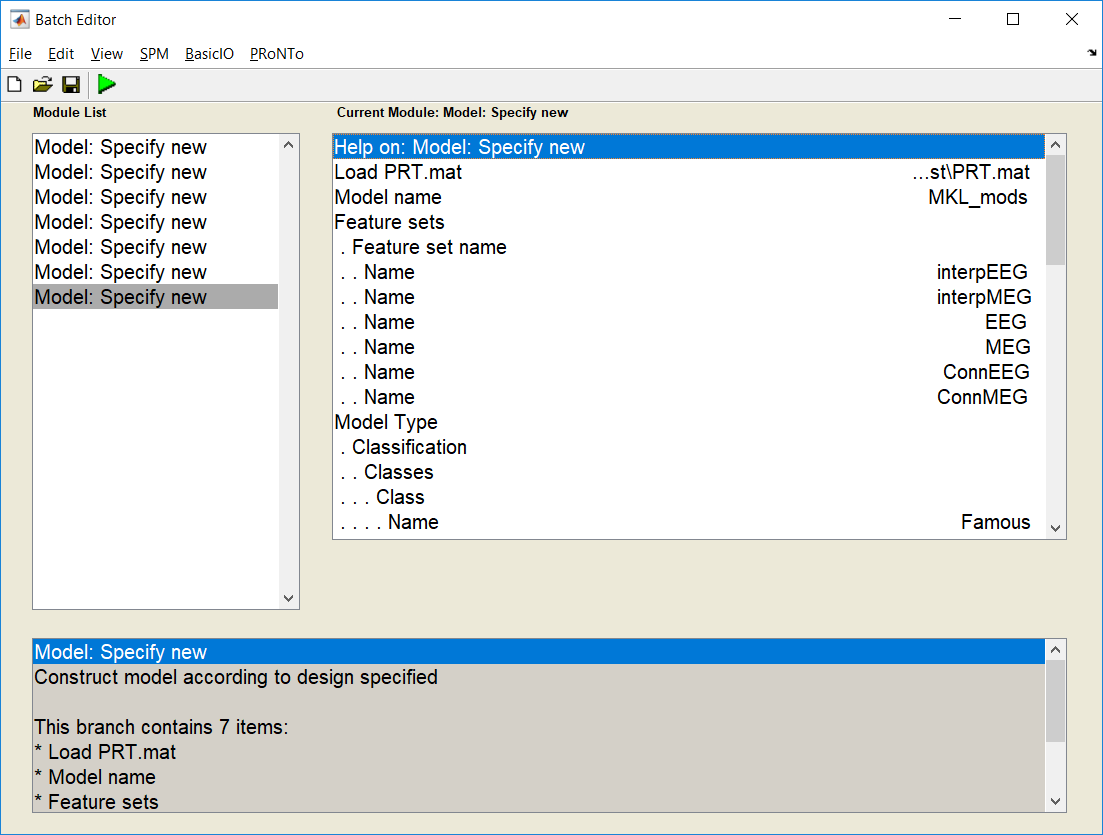
\includegraphics[scale=0.5]{images/Tutorial/v3/multimodal_face_tutorial/multimodal_face_batch_model_specify_new_all.png}
	\caption{All 7 {\tt matlabbatch} `Model: Specify new' modules.}
	\label{fig:multimodal_face_batch_model_specify_new_all}
\end{figure}

%------------------------------------------------------------------

\subsection{Model: Run}

\begin{itemize}

	\item Click on the `Model: Run' option on PRoNTo's {\tt matlabbatch} menu.
	
	\item Select the appropriate `PRT.mat' file, either manually, or if you have all modules together in the `Module List' using the Dependency button to associate it with the module of the previous step.
	
	\item Select the model name from the first `Model: Specify new' module with the `Dependency' button, or write it {\it exactly}, as previously defined in the `Model: Specify new' module, here `interpEEG\_SVM'.

	\item In the `Do permutation test?' select `Permutation test', with 100 repetitions. Be aware that 100 repetitions is a small number when running permutation tests, and 1000 repetitions (or even more) is a more realistic one if you want your results to have a good statistical power.
	
\end{itemize}

Figure \ref{fig:multimodal_face_batch_model_run_final} shows the final configuration of the {\tt matlabbatch} `Model: Run' module.

\begin{figure}[!h]
	\centering
		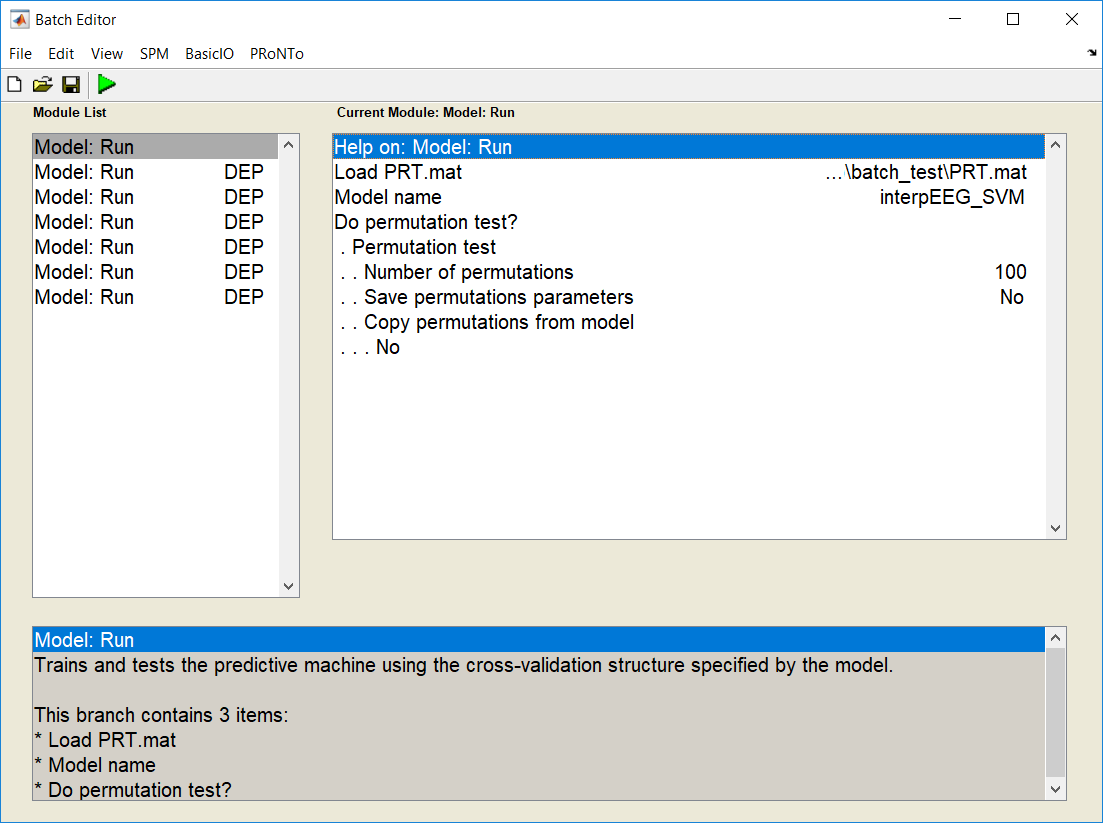
\includegraphics[scale=0.5]{images/Tutorial/v3/multimodal_face_tutorial/multimodal_face_batch_model_run_final.png}
	\caption{The {\tt matlabbatch} `Model: Run' modules.}
	\label{fig:multimodal_face_batch_model_run_final}
\end{figure}

\noindent Follow the same procedure (as in the previous section) by replicating the now finished `Model: Run' module 6 more times, each time changing only the name of the model to be run. Remember that we have 7 models in total, 6 single kernel models and 1 multi-kernel model.

%------------------------------------------------------------------

\subsection{Compute weights}

\begin{itemize}

	\item Click on the `Compute weights' option on PRoNTo's {\tt matlabbatch} menu.

	\item With `Load PRT.mat' field selected, click on the `Dependency' button to associate the `PRT.mat' file created in the previous step, or locate the `PRT.mat' manually.
	
	\item It's optional to define an image name.
	
	\item Finally, set the `Build weights images for permutations' field to `No'. 

\end{itemize}

\noindent As we did before, replicate this module 6 times. Each time you will only need to change the name of the model (either set it manually, or associate it properly using the `Dependency' button, if you have all modules in the module list) so that we compute weights for all 7 models. Figure \ref{fig:multimodal_face_batch_compute_weights_final} shows the final configuration of the {\tt matlabbatch} `Compute weights' module.
\\

\begin{figure}[!h]
	\centering
		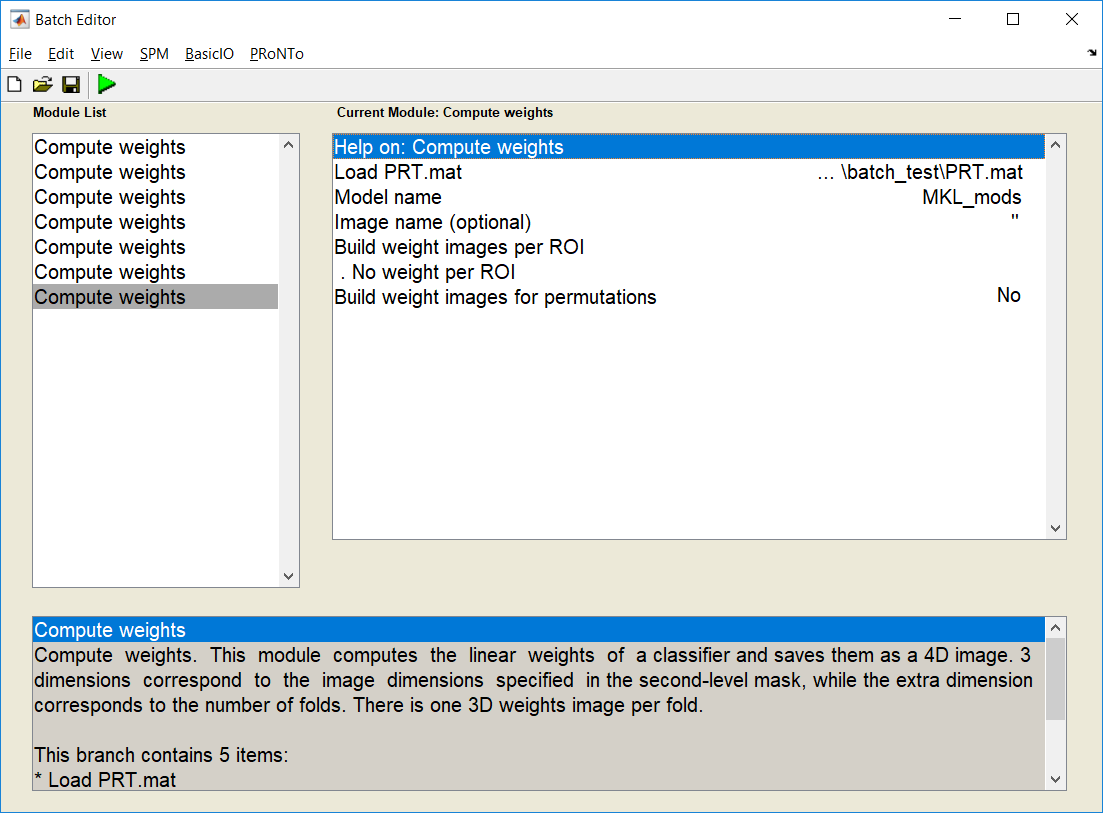
\includegraphics[scale=0.5]{images/Tutorial/v3/multimodal_face_tutorial/multimodal_face_batch_compute_weights_final.png}
	\caption{Final configuration of the {\tt matlabbatch} `Compute weights' module.}
	\label{fig:multimodal_face_batch_compute_weights_final}
\end{figure}

It is advised that you save the batches, either in groups or if possible all together, so that you can open and edit them for further analyses.

%------------------------------------------------------------------

\subsection{Display results \& weights}

If everything was set properly, the results should be the same as those obtained using GUI.

\subsection{Using an atlas with .mat}

The changes needed to use an atlas with .mat, compared to not using an atlas, are straight forward, and the reader is referred to \ref{ssec:atlas_w_mat} where the same procedure is followed.

% \ref{sec:mkl_Batch_analysis} XXXX